\chapter{Forelesninger}
\sloppy

\section{Forelesning 8 (Tirsdag 28. januar 2025)}

\begin{theorem}{Lax-Equivalence-Theorem}{}
  \[
    \text{Consistency} + \text{Stability} \iff \text{Convergence}
  \]
  Holds for linear (time-dependent) problems.
\end{theorem}

PDE:

\begin{align*}
  u_t + u_x  = au, \quad \R \\
  u(x, 0) = f(x) \tag{IC}   \\
  u(0, t) = g(t) \tag{BC}   \\
  u(x,t) =
  \begin{cases}
    e^{at}f(x-t), & x < t \\
    e^{at}g(t-x), & x > t
  \end{cases}
\end{align*}

\paragraph{Scheme:}
\begin{align*}
  U_m^{n+1} = U_m^n - \frac{K}{h}(U_m^n - U_{m-1}^n) + aKU_m^n \\
  \tau_m^n = \frac{1}{2}(K\partial_t^2 u_m^n - h\partial_x^2 u_m^n) + O(K^2 + h^2)
\end{align*}

\[
  \norm{\vec{\tau}^n} \underset{h, K \to 0}{\longrightarrow} 0 \tag{Consistency}
\]

\paragraph{Stencil:}
\begin{figure}[H]
  \centering
  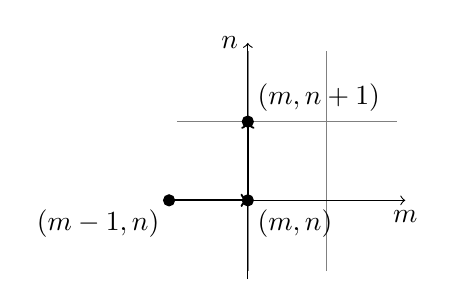
\begin{tikzpicture}
    \draw[step=1cm,gray,very thin] (-0.9,-0.9) grid (1.9,1.9);
    \draw[->] (-1,0) -- (2,0) node[below] {$m$};
    \draw[->] (0,-1) -- (0,2) node[left] {$n$};
    \filldraw[black] (0,0) circle (2pt) node[below right] {$(m,n)$};
    \filldraw[black] (-1,0) circle (2pt) node[below left] {$(m-1,n)$};
    \filldraw[black] (0,1) circle (2pt) node[above right] {$(m,n+1)$};
    \draw[->,thick] (0,0) -- (0,1);
    \draw[->,thick] (-1,0) -- (0,0);
  \end{tikzpicture}
  \caption{Stencil}
  \label{fig:stencil}
\end{figure}

\paragraph{Stability:}
Find \(C\). Define \( S = \frac{K}{h} \).

\[
  U_m^{n+1} = (1 - S + aK)U_m^n + SU_{m-1}^n
\]

\[
  \begin{bmatrix}
    U_1^{n+1} \\
    U_2^{n+1} \\
    \\
    \vdots    \\
    \\
    U_M^{n+1}
  \end{bmatrix}
  =
  \begin{bmatrix}
    1 - S + aK & 0          & 0          & \cdots & 0          \\
    S          & 1 - S + aK & 0          & \cdots & 0          \\
    0          & S          & 1 - S + aK & \cdots & 0          \\
    \vdots     & \vdots     & \vdots     & \ddots & \vdots     \\
    0          & \cdots     & 0          & S      & 1 - S + aK
  \end{bmatrix}
  \begin{bmatrix}
    U_1^n  \\
    U_2^n  \\
    \\
    \vdots \\
    \\
    U_M^n
  \end{bmatrix}
  +
  \begin{bmatrix}
    \overbrace{S g(t_0)}^{U_0^n} \\
    0                            \\
    \vdots                       \\
    0                            \\
    \overbrace{S g(t_n)}^{U_{M+1}^n}
  \end{bmatrix}
\]

\begin{example}{}{}
  \begin{align*}
    u_t = u_{xx} \text{ on } [0,1] \\
    u(x, 0) = f(x)                 \\
    u(1, t) = 0                    \\
    u(0, t) + u_x(0, t) = 0
  \end{align*}
  \paragraph{Scheme}
  let \( r= \frac{K}{h^2} \)
  \[
    U_m^{n+1} = U_m^n + r(U_{m-1}^n - 2U_m^n + U_{m+1}^n)
  \]
  \paragraph{Boundary Conditions}
  \begin{align*}
    U_0^{n+1} = U_0^n + r(U_1^n - 2U_0^n + U_{-1}^n)        \\
    U_0^n + \frac{1}{2h}(U_1^n - U_{-1}^n) = 0              \\
    U_{-1}^n = U_1^n + 2hU_0^n                              \\
    U_0^{n+1} = U_0^n + r(U_1^n - 2U_0^n + U_1^n + 2hU_0^n) \\
    U_0^{n+1} = U_0^n + r(2U_1^n - 4U_0^n)                  \\
    U_0^{n+1} = U_0^n + 2rU_1^n - 4rU_0^n                   \\
    U_0^{n+1} = (1 - 2r(1 - h))U_0^n + 2rU_1^n
  \end{align*}
  Let \( \vec{U}^n = \begin{bmatrix} U_0^n \\ U_1^n \\ \vdots \\ U_M^n \end{bmatrix} \) where \( U_M^n = 0 \).

  \[
    C = \begin{bmatrix}
      1 - 2r(1 - h) & 2r     & 0      & \cdots & 0      \\
      r             & 1 - 2r & r      & \cdots & 0      \\
      0             & r      & 1 - 2r & \cdots & 0      \\
      \vdots        & \vdots & \vdots & \ddots & \vdots \\
      0             & \cdots & 0      & r      & 1 - 2r
    \end{bmatrix}
  \]

  Need to find \( r \leq \frac{1}{2} \) for \(m = 1, 2, \ldots, M-1\) to ensure stability.
  For \( m = 0 \) we need:
  \begin{align*}
    \abs{1 - 2r(1 - h)} + \abs{2r} \leq 1 + \mu K \\
    \abs{1 - 2r(1 - h)} + 2r \leq \abs{1 - 2r} + 2rh + \abs{2r} = 1 + 2rh = 1 + \underbrace{\frac{2}{h}}_{\mu}K
  \end{align*}
  Stable for a given \( h \) but not when \( h \to 0 \).
  \begin{align*}
    K \tau_0^n =                              & u(0, t_n + h) - u(0, t_n) + 2r(1 - h)u(0, t_n) - 2ru(h, t_n)                                                                                                                                            \\                                                                                                                                                                                                                    \\
    =            u_0^n + K \partial_t u_0^n + & \frac{1}{2}K^2 \partial_t^2 u_0^n + \ldots - u_0^n                                                                                                                                                      \\
    +                                         & 2\frac{K}{h^2}(1 - h)u_0^n - 2\frac{K}{h^2}(u_0^n + h \partial_x u_0^n + \frac{1}{2}h^2 \partial_x^2 u_0^n + \frac{1}{6}h^3 \partial_x^3 u_0^n + \frac{1}{24}h^4 \partial_x^4 u_0^n + \ldots)           \\
                                              & = \frac{K}{h^2}\left[-h(u_0^n + \partial_x u_0^n)\right] + K \left[\partial_t u_0^n - \partial_x^2 u_0^n\right] - \frac{1}{3}Kh\partial_x^3 u_0^n + \ldots + \frac{1}{2}K^2 \partial_t^2 u_0^n + \ldots \\
    K \tau_0^n                                & = -\frac{1}{3}Kh\partial_x^3 u_0^n + \ldots + \frac{1}{2}K^2 \partial_t^2 u_0^n + \ldots \tag{Consistency}
  \end{align*}
\end{example}

\paragraph{Alternative stability analysis: Von Neumann analysis}
Von Neumann analysis is a method for analyzing the stability of finite difference schemes for linear partial differential equations.
The method is based on the Fourier analysis of the numerical solution.

\begin{theorem}{Parseval's equality}{}
  \[
    \sum_{l=-\infty}^{\infty} \abs{C_l}^2 = \frac{1}{2\pi} \int_0^{2\pi} \abs{f(x)}^2 \dd{x}
  \]
\end{theorem}

\begin{example}{}{}
  \begin{align*}
    u_t = u_{xx} \text{ on } [0,1] \\
    u(x, 0) = f(x)                 \\
  \end{align*}
  Make a periodic extension of \(f\), s.t. \(f(x) = f(x-1)\).
  Assue that \(u(x-1, t) = u(x, t)\) and \(u(1, t) = u(0, t)\).
  Write \(f(x)\) as a complex Fourier series:
  \begin{align*}
    f(x) & = \sum_{k=-\infty}^{\infty} C_l e^{i \beta_l x}, \quad \beta_l = 2\pi l, \quad l \in \Z \\
    C_l  & = \int_0^1 f(x) e^{-i \beta_l x} \dd{x}
  \end{align*}

  Seperation of variables:
  \[
    u_l(x, t) = e^{-\beta_l^2 t} e^{i \beta_l x}
  \]
  Plug in the (IC):
  \[
    u(x, t) = \sum_{l=-\infty}^{\infty} C_l e^{-\beta_l^2 t} e^{i \beta_l x}
  \]
  \subparagraph{Idea}
  Given a scheme for \(u_t = u_{xx}\), we can write:
  \[
    U_m^{n+1} = U_m^n + r(U_{m-1}^n - 2U_m^n + U_{m+1}^n), \quad r = \frac{k}{h^2}
  \]

  Search for a solution of the form:
  \[
    U_m^n = \psi^n e^{i \beta x_m}
  \]
  A scheme is \textit{Von Neumann stable} if:
  \[
    \abs{\psi} < 1 + \mu k, \quad \mu \geq 0
  \]

  In our example:
  \begin{align*}
    \psi^{n+1} e^{i \beta x_m} & = \psi^n e^{i \beta x_m} + r\psi^n\left(e^{i \beta x_{m+1}} - 2e^{i \beta x_m} + e^{i \beta x_{m-1}}\right)           \\
                               & = \psi^n e^{i \beta x_m} (1 + r(e^{i \beta h} - 2 + e^{-i \beta h}))                                                  \\
    \psi                       & = 1 + r(e^{i \beta h} - 2 + e^{-i \beta h})                                                                           \\
                               & = 1 + r(2\cos(\beta h) - 2)                                                                                           \\
                               & = 1 + 4r\sin^2\left(\frac{\beta h}{2}\right)                                                                          \\
    \abs{\psi}                 & = \abs{1 + 4r\sin^2\left(\frac{\beta h}{2}\right)} \leq 1 \iff r \leq \frac{1}{2}, \forall \beta \text{ and } \mu = 0
  \end{align*}
\end{example}
\section{Forelesning 9 (Mandag 3. februar 2025)}

\paragraph{Von Neumann Stability Analysis}

\begin{itemize}
  \item Let \( U_m^n = \xi^n e^{i\beta m} \). Insert this into Difference Equation (DE).
  \item The method is Von Neumann Stable if \( \abs{\xi} \leq 1 + \mu K \) for all \( \beta \).
  \item Von Neumann stability is sufficient and necessary for pure IVP problems (Cauchy problems).
\end{itemize}
\begin{figure}[H]
  \centering
  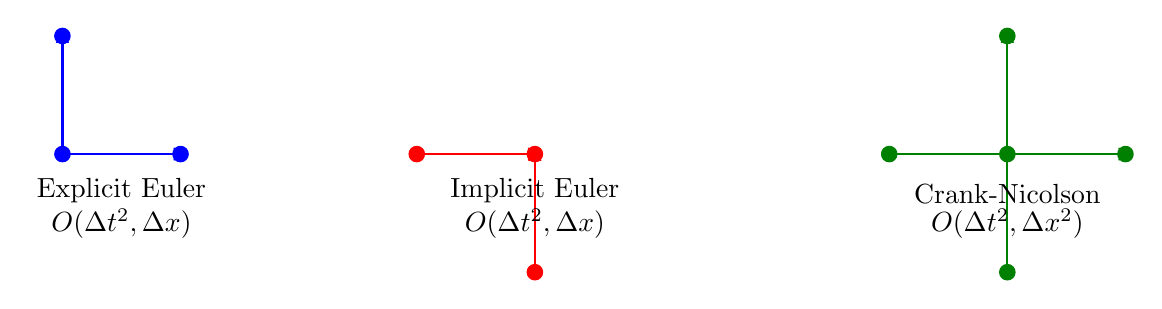
\begin{tikzpicture}[scale=1.5]
    % Explicit Euler (Forward)
    \begin{scope}[xshift=0cm]
      \fill[blue] (0,0) circle (2pt);
      \fill[blue] (0,1) circle (2pt);
      \fill[blue] (1,0) circle (2pt);
      \draw[->,thick,blue] (0,0) -- (1,0);
      \draw[->,thick,blue] (0,0) -- (0,1);
      \node[above] at (0.5,-0.5) {Explicit Euler};
      \node[above] at (0.5,-0.8) {\(O(\Delta t^2, \Delta x)\)};
    \end{scope}

    % Implicit Euler (Backward)
    \begin{scope}[xshift=4cm]
      \fill[red] (0,0) circle (2pt);
      \fill[red] (-1,0) circle (2pt);
      \fill[red] (0,-1) circle (2pt);
      \draw[->,thick,red] (-1,0) -- (0,0);
      \draw[->,thick,red] (0,-1) -- (0,0);
      \node[above] at (0,-0.5) {Implicit Euler};
      \node[above] at (0,-0.8) {\(O(\Delta t^2, \Delta x)\)};
    \end{scope}

    % Crank-Nicolson
    \begin{scope}[xshift=8cm]
      \fill[green!50!black] (0,0) circle (2pt);
      \fill[green!50!black] (1,0) circle (2pt);
      \fill[green!50!black] (-1,0) circle (2pt);
      \fill[green!50!black] (0,1) circle (2pt);
      \fill[green!50!black] (0,-1) circle (2pt);
      \draw[->,thick,green!50!black] (-1,0) -- (1,0);
      \draw[->,thick,green!50!black] (0,-1) -- (0,1);
      \node[above] at (0,-0.5) {Crank-Nicolson};
      \node[above] at (0,-0.8) {\(O(\Delta t^2, \Delta x^2)\)};
    \end{scope}
  \end{tikzpicture}
  \caption{Stencils for different numerical schemes}
  \label{fig:stencils}
\end{figure}



\begin{example}{Heat equation}{}
  \[
    u_t = u_{xx}, \quad 0 \leq x \leq 1, \quad 0 \leq t \leq 0.5
  \]
  \[
    \begin{cases}
      u(x, 0) = \sin(\pi x) \\
      u(0, t) = u(1, t) = 0
    \end{cases}
  \]
  \[
    u(x, t) = \sin(\pi x) e^{-\pi^2 t}
  \]

  \subparagraph{Finite Difference Scheme}
  \[
    \frac{1}{2k}\left( U_m^{n+1} - U_m^{n-1} \right) = \frac{1}{h^2}\left( U_{m-1}^n - 2U_m^n + U_{m+1}^n \right)
  \]

  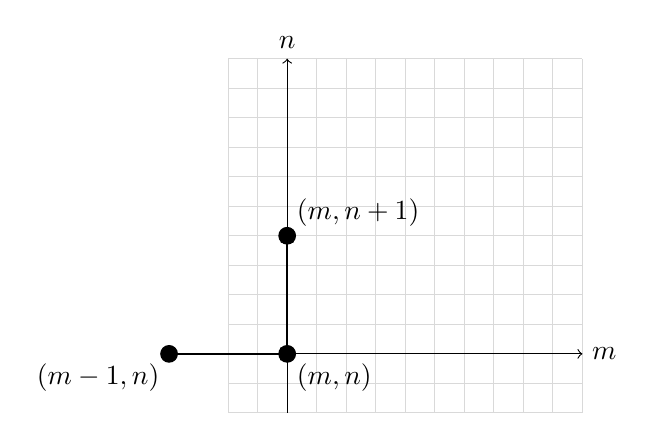
\begin{tikzpicture}[scale=1.5]
    % Grid
    \draw[step=0.25cm,gray!30] (-0.5,-0.5) grid (2.5,2.5);
    \draw[->] (-0.5,0) -- (2.5,0) node[right] {$m$};
    \draw[->] (0,-0.5) -- (0,2.5) node[above] {$n$};
    % Points
    \filldraw[black] (0,0) circle (2pt) node[below right] {$(m,n)$};
    \filldraw[black] (-1,0) circle (2pt) node[below left] {$(m-1,n)$};
    \filldraw[black] (0,1) circle (2pt) node[above right] {$(m,n+1)$};
    % Arrows
    \draw[->,thick] (0,0) -- (0,1);
    \draw[->,thick] (-1,0) -- (0,0);

  \end{tikzpicture}


  \subparagraph{Fourier Stability Analysis}

  \begin{align*}
    U_m^{n+1}
     & =
    2r\left( U_{m-1}^n - U_m^n + U_{m+1}^n \right) + U_m^{n-1}               \\
    \xi^{n+1} e^{i\beta x_m}
     & =
    2r\xi^n
    \left[
      e^{i\beta x_m - h} - 2e^{i\beta x_m} + e^{i\beta x_m + h}
      \right]
    + \xi^{n-1} e^{i\beta x_m}                                               \\
    \xi^2
     & =
    2r\left[ e^{-i\beta h} - 2 + e^{i\beta h} \right]\xi + 1                 \\
    \xi^2
     & =
    2r \left[ 2\cos(\beta h) - 2 \right]\xi+ 1                               \\
    \xi^2 + 8r\sin^2 \frac{\beta h}{2}\xi - 1
     & =
    0 \quad  \implies \quad \xi_\pm
    =
    -4r\sin^2 \frac{\beta h}{2} \pm \sqrt{16r^2\sin^4 \frac{\beta h}{2} + 1} \\
    \xi_- \leq - 1
    \quad
    \abs{\xi_-} \leq 1
  \end{align*}

  \textbf{Conclusion:} The scheme is unconditionally unstable.

  But we can stabilize the scheme by introducing a damping term (Du Fort-Frankel scheme):
  Replace \( U_m^n \leftarrow \frac{1}{2}(U_m^{n+1} + U_m^{n-1}) \) in the scheme.

  \begin{align*}
    \frac{1}{2k}\left( U_m^{n+1} - U_m^{n-1} \right)
     & =
    \frac{1}{h^2}\left( U_{m-1}^n + U_{m+1}^n\right) - \frac{1}{h^2}\left( U_m^{n+1} + U_m^{n-1} \right) \\
    (1 + 2r)U_m^{n+1}
     & =
    2r\left( U_{m-1}^n + U_{m+1}^n \right) + (1 - 2r)U_m^{n-1}                                           \\
    (1 + 2r)\xi^2 - 4r \cos \beta h \xi - (1 - 2r)
     & = 0                                                                                               \\
    \xi_\pm
     & = \frac{1}{1 + 2r} \left[ 2r\cos \beta h \pm \sqrt{4r^2\cos^2 \beta h + (1 - 2r)(1 + 2r)} \right] \\
    \xi_\pm
     & = \frac{1}{1 + 2r} \left[ 2r\cos \beta h \pm \sqrt{1 - 4r^2 \sin^2 {bh}} \right]                  \\
    \abs{\xi_\pm}^2 = \frac{2r - 1}{2r + 1} < 1 \quad \text{for all } r                                  \\
  \end{align*}

  \textbf{Conclusion:} The method scheme is unconditionally stable, for all \( r \).

  Now we know that the scheme has stability for all \( r \), it might still not converge because we also need consistency.

  \subparagraph{Consistency}
  \begin{align*}
    \tau_m^n & = \frac{1}{2k}\left( u_m^{n+1} - u_m^{n-1} \right)                                               \\
             & - \frac{1}{h^2}\left( u_{m-1}^n - u_{m+1}^n \right)                                              \\
             & + \frac{1}{h^2}\left( u_m^{n+1} - u_m^{n-1} \right)                                              \\
             & =                                                                                                \\
             & \frac{1}{2k}\left[ 2k u_t + 2k^3 \frac{1}{3!}u_{tt} + \ldots \right]                             \\
             & -\frac{1}{h^2}\left[ 2u + 2h^2 \frac{1}{2!}u_{xx} + 2h^4 \frac{1}{4!}u_{xxxx} + \ldots \right]   \\
             & + \frac{1}{h^2}\left[ 2 u + 2k^2 \frac{1}{2!}u_{tt} + 2k^4 \frac{1}{4!}u_{tttt} + \ldots \right] \\
             & =
    u_t - u_xx
    + \frac{k^2}{h^2}u_{tt} + \frac{k^2}{3!}u_{tt}
    + \frac{h^2}{12}u_{xxxx} + \frac{k^4}{12h^2}u_{tttt}
    + \ldots
  \end{align*}
  The method is consistent only if the truncation error goes to zero as \( h, k \to 0 \).

  Here the method is consistent when \(\frac{k}{h} \underset{h,k \to 0}{\longrightarrow} 0\).

  \textbf{Conclusion:} The method is conditionally consistent.

  \textbf{Conclusion:} The method is conditionally stable and consistent for all \( r \) and \( \frac{k}{h} \underset{h,k \to 0}{\longrightarrow} 0 \) and therefore convergent.

\end{example}

\paragraph{Domain of dependence}

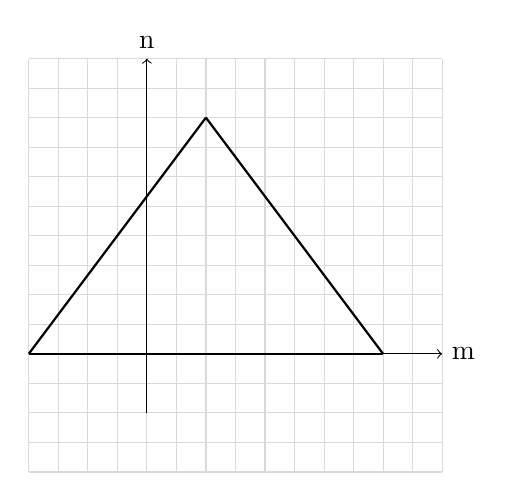
\begin{tikzpicture}[scale=1.5]
  % Grid
  \draw[step=0.25cm,gray!30] (-1,-1) grid (2.5,2.5);
  \draw[->] (-1,0) -- (2.5,0) node[right] {m};
  \draw[->] (0,-0.5) -- (0,2.5) node[above] {n};

  % Triangle
  \draw[-,thick] (-1,0) -- (0.5,2);
  \draw[-,thick] (-1,0) -- (2,0);
  \draw[-,thick] (2,0) -- (0.5,2);

\end{tikzpicture}
\section{Forelesning 10 (Tirsdag 4. februar 2025)}

\paragraph{Hyperbolic PDEs}

\begin{align*}\label{eq:hb1}
  a u_{xx} + 2bu_{xy} + c u_{yy} = f(x,y, u, u_x, u_y) \tag{1} \\
  \begin{cases}
    b^2 - ac > 0 & \text{Hyperbolic} \\
    b^2 - ac = 0 & \text{Parabolic}  \\
    b^2 - ac < 0 & \text{Elliptic}
  \end{cases}                             \\
\end{align*}

\begin{example}{Wave equation}{}
  \begin{align*}
    u_{tt} & = c^2 u_{xx}                                                                                   \\
    u(x,0) & = f(x), \quad u_t(x,0) = g(x)                                                                  \\
    u(x,t) & = \frac{1}{2}\left[ f(x - ct) + f(x + ct) \right] + \frac{1}{2c} \int_{x-ct}^{x+ct} g(s) \, ds
  \end{align*}
\end{example}

\subparagraph{D'Alembert's principle}
\begin{figure}[H]
  \centering
  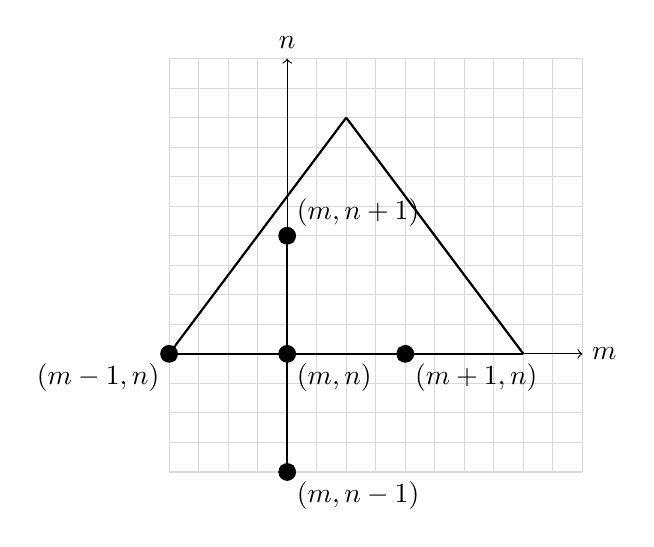
\begin{tikzpicture}[scale=1.5]
    % Grid
    \draw[step=0.25cm,gray!30] (-1,-1) grid (2.5,2.5);
    \draw[->] (-1,0) -- (2.5,0) node[right] {$m$};
    \draw[->] (0,-0.5) -- (0,2.5) node[above] {$n$};

    % Triangle
    \draw[-,thick] (-1,0) -- (0.5,2);
    \draw[-,thick] (-1,0) -- (2,0);
    \draw[-,thick] (2,0) -- (0.5,2);

    % Points
    \filldraw[black] (0,0) circle (2pt) node[below right] {$(m,n)$};
    \filldraw[black] (-1,0) circle (2pt) node[below left] {$(m-1,n)$};
    \filldraw[black] (0,1) circle (2pt) node[above right] {$(m,n+1)$};
    \filldraw[black] (1,0) circle (2pt) node[below right] {$(m+1,n)$};
    \filldraw[black] (0,-1) circle (2pt) node[below right] {$(m,n-1)$};

    % Arrows
    \draw[->,thick] (0,0) -- (0,1);
    \draw[->,thick] (0,0) -- (1,0);
    \draw[->,thick] (0,0) -- (-1,0);
    \draw[->,thick] (0,0) -- (0,-1);

  \end{tikzpicture}
  \caption{Stencils for the wave equation}
  \label{fig:wave-stencils}
\end{figure}

\begin{align*}
  Lu          & = \partial_t^2 u - c^2 \partial_x^2 u = (\partial_t - c \partial_x)(\partial_t + c \partial_x)u = 0 \\
  u_t + c u_x & = v                                                                                                 \\
  v_t - c v_x & = 0
\end{align*}

\subparagraph{1st order equations}
\begin{itemize}
  \item Density: \(u\)
  \item Non-conservative:
        \begin{equation}
          \label{eq:hb2}
          u_t + a(x,t,u)u_x = b(x,t,u)
        \end{equation}
  \item Transport equation: \(u_t + au_x = 0\) where \(a\) is a constant.
        \[
          \dd{t} \int_{x_1}^{x_2} u(x,t) \, dx = \int_{x_1}^{x_2} u_t(x,t) \, dx = -\int_{x_1}^{x_2} (f(u))_x \, dx = f(u(x_1,t)) - f(u(x_2,t))
        \]
  \item Conservation laws: \(u_t + (f(u))_x = 0\)
\end{itemize}

\subparagraph{1st order system}
\begin{itemize}
  \item Non-conservative:
        \[
          \label{eq:hb3}
          \symbf{u_t} + A(\symbf{u}_x) = \symbf{b}\tag{3}
        \]
  \item Conservative: \[\symbf{u_t} + (\symbf{f}(\symbf{u}))_x = 0\]
        This is hyperbolic if \(A\) is diagonalizable with real eigenvalues.
        \[
          A = PDP^{-1} \quad \text{where} \quad D = \text{diag}(\lambda_1, \ldots, \lambda_n)
        \]
        Equivalently, if the Jacobian matrix of \(\symbf{f}\) is diagonalizable with real eigenvalues.

        For linear problems (Hyperbolic PDEs),\eqref{eq:hb1} can always be written as \eqref{eq:hb3}.
        \eqref{eq:hb3} can always be decoupled into a set of \eqref{eq:hb2} equations.
\end{itemize}
\paragraph{Method of Characteristics}
Let \(u_t + a(x,t,u)u_x = b(x,t,u)\) be a non-conservative hyperbolic PDE. Furthermore let \(v(t) = u(x(t), t)\) where \(x(t)\) is a characteristic curve. Then
\[
  \dot{v} = u_x \dot{x} + u_t = u_t + a(x,t,u)u_x = b(x(t), t, u(x(t), t)=v(t))
\]
Let \(\dot{x} = a(x,t,u)\) (characteristic equation) and \(\dot{v} = b(x(t), t, v(t))\) (System of ODEs).
Initial values: \(\begin{cases} x(t_0) = x_0 \\ v(t_0) = u(x_0, t_0) \end{cases}\) is known for all \((t_0, x_0)\) on the initial curve.

\begin{align*}
  x(t) & = \mathcal{X}(t; t_0, x_0), \quad x_0 = x(t_0) = \mathcal{X}^{-1}(x, t)               \\
  v(t) & = \mathcal{V}(t; x_0, t_0, u_0), \quad u(x,t) = \mathcal{V}(t, \mathcal{X}^{-1}(x,t))
\end{align*}

\begin{example}{}{}
  \(u_t + a u_x = b\) where \(a, b\) can be functions of \(x, t, u\)
  \begin{align*}
    u_t + a(x,t,u)u_x      & = b(x,t,u)                                           \\
    u(x,0)                 & = u_0(x)   \quad \Sigma \text{ is the initial curve} \\
    \dot{x(t)}        = a, & \quad x(0) = x_0                                     \\
                           & \implies x(t) = x_0 + at                             \\
                           & \implies x_0 = x - at                                \\
                           & \implies u(x_0, 0) = u_0(x_0) \text{ is known}       \\
    \dot{v(t)}             & = b
  \end{align*}

  % FYLL FRA BILDER PÅ TLF!

\end{example}


\subparagraph{Finite Difference Scheme}
\[
  \frac{1}{k^2}\left( U_m^{n+1} - 2U_m^n + U_m^{n-1} \right) = \frac{1}{h^2}\left( U_{m-1}^n - 2U_m^n + U_{m+1}^n \right)
\]

\subparagraph{Von Neumann Stability Analysis}
\begin{align*}
  U_m^n         & = \xi^n e^{i\beta m}                                                    \\
  \xi^2         & = \frac{1}{r^2} - 2 + \frac{1}{r^2} = 2\left( \frac{1}{r^2} - 1 \right) \\
  \xi_\pm       & = \pm \sqrt{2\left( \frac{1}{r^2} - 1 \right)}                          \\
  \abs{\xi_\pm} & \leq 1 \quad \text{if} \quad r \geq 1
\end{align*}

\textbf{Conclusion:} The method is conditionally stable.

\subparagraph{Consistency}
\[
  \tau_m^n = \frac{1}{k^2}\left( u_t - u_{xx} \right) + O(k^2, h^2)
\]

\textbf{Conclusion:} The method is consistent.

\textbf{Conclusion:} The method is conditionally stable and consistent and therefore convergent.


\begin{example}{}{}

  \[
    u_t + e^{-x}u_x = 0, \quad u(x,0) = u_0(x)
  \]

  \textbf{Method of Characteristics:}
  \begin{align*}
    \dot{x} & = e^{-x}, \quad x(0) = x_0             \\
    \dot{v} & = 0, \quad v(0) = u(x_0, 0) = u_0(x_0)
  \end{align*}
  \begin{align*}
    \frac{dx}{dt} = e^{-x} & \implies \int_{x_0}^x e^x \, dx = \int_0^t \, dt \implies e^x - e^{x_0} = t \implies x_0 = \ln(e^x - t) \\
    \frac{dv}{dt} = 0      & \implies v = u_0(x_0) = u_0(\ln(e^x - t))
  \end{align*}

\end{example}
\section{Forelesning 11 (Mandag 10. februar 2025)}

\paragraph{What about systems?}

\begin{align*}
  \symbf{u_t} + A(\symbf{u}_x)                          & = \symbf{0} \\
  \symbf{u_t} + P\Lambda P^{-1}(\symbf{u}_x)            & = \symbf{0} \\
  P^{-1}\symbf{u_t} + \Lambda P^{-1}\Lambda(symbf{u}_x) & = \symbf{0} \\
  \symbf{v_t} + \Lambda \symbf{v}_x                     & = \symbf{0}
\end{align*}

Hyperbolic if \(A\) is diagonalizable with real eigenvalues: \(A = P\Lambda P^{-1}\) where \(\Lambda = \text{diag}(\lambda_1, \ldots, \lambda_n)\).

\begin{example}{}{}
  \begin{align*}
    \symbf{v_{i,t} + \lambda_i v_{i,x} = 0}                                     \\
    \symbf{u}_t +
    \begin{bmatrix}
      a & b \\
      c & d
    \end{bmatrix}
    \symbf{u}_x = \symbf{0} \quad \text{where} \quad x\in [0,1], \quad t \geq 0 \\
    \symbf{u}(x,0) = \symbf{f}(x) \quad \text{is the initial curve}
  \end{align*}

  Then the eigenvalues are \(\lambda_{1,2} = a \pm b\) with eigenvectors
  \[
    P = \begin{bmatrix}
      1 & 1  \\
      1 & -1
    \end{bmatrix}
  \]
  and
  \[
    \symbf{v} = P^{-1}\symbf{u} \implies \symbf{u} = P\symbf{v}
  \]

  then we get the system

  \begin{align*}
    \symbf{v}_{1,t} + (a + b)\symbf{v}_{1,x} & = 0 \\
    \symbf{v}_{2,t} + (a - b)\symbf{v}_{2,x} & = 0
  \end{align*}

  assume that \(a > 0\), with the BCs
  \[
    x=0 \quad \text{inflow if } \lambda > 0 \quad \vee quad x = 1 \quad \text{outflow if } \lambda < 0
  \]

  \subparagraph{Case 1}
  \[
    a > b \quad \text{and} \quad \lambda_1, \lambda_2 > 0
  \]



\end{example}


\paragraph{Scheming}
\[
  \symbf{u}_t + a \symbf{u}_x = 0 , \quad b \in \R \quad \symbf{u}(x,0) = \symbf{f}(x)
\]

%draw Grid
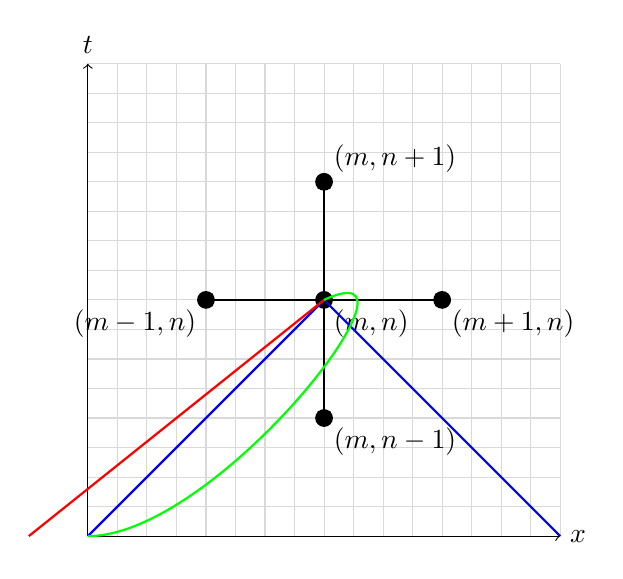
\begin{tikzpicture}[scale=1.5]
  % Grid
  \draw[step=0.25cm,gray!30] (-1,-1) grid (3,3);
  \draw[->] (-1,-1) -- (3,-1) node[right] {$x$};
  \draw[->] (-1,-1) -- (-1,3) node[above] {$t$};

  % Points
  \filldraw[black] (1,1) circle (2pt) node[below right] {$(m,n)$};
  \filldraw[black] (0,1) circle (2pt) node[below left] {$(m-1,n)$};
  \filldraw[black] (1,2) circle (2pt) node[above right] {$(m,n+1)$};
  \filldraw[black] (2,1) circle (2pt) node[below right] {$(m+1,n)$};
  \filldraw[black] (1,0) circle (2pt) node[below right] {$(m,n-1)$};

  % Stencils
  \draw[->,thick] (1,1) -- (1,2);
  \draw[->,thick] (1,1) -- (2,1);
  \draw[->,thick] (1,1) -- (0,1);
  \draw[->,thick] (1,1) -- (1,0);

  % Stencil 2 (Orange)
  \draw[-,thick,blue] (-1,-1) -- (1,1);
  \draw[-,thick,blue] (3,-1) -- (1,1);

  % Stencil 3 (red, outside)
  \draw[-,thick,red] (-1.5,-1) -- (1,1);

  % Stencil 4 (green, curved inside)
  \draw[-,thick,green] (-1,-1) to [out=0,in=25] (1,1);



\end{tikzpicture}

\subparagraph{Central Time, Central Space}
\[
  \frac{1}{k}\left( U_m^{n+1} - U_m^{n-1} \right) = \frac{1}{h}\left( U_{m+1}^n - U_{m-1}^n \right)
\]

\subparagraph{Forward Time, Central Space}
\[
  \frac{1}{k}\left( U_m^{n+1} - U_m^n \right) = \frac{1}{h}\left( U_{m+1}^n - U_{m-1}^n \right)
\]

´
Then
\[
  U_m^{n+1} = \beta_{-1} U_{m-1}^n + \beta_0 U_m^n + \beta_1 U_{m+1}^n
\]

Assume that \(\beta_{-1} \neq 0\) and \(\beta_1 \neq 0\), then the method is unconditionally unstable.

\begin{align*}
  T = k n                                                     \\
  x_{m-n} = \mathcal{X} - \dfrac{T}{k}h = \mathcal{X} - \mu T \\
  x_{m+n} = \mathcal{X} + \dfrac{T}{k}h = \mathcal{X} + \mu T
\end{align*}

Interval of dependence: \(\left[ \mathcal{X} - \mu T, \mathcal{X} + \mu T \right]\)

Domain of dependence: Triangle of this and \((X,T)\).

\subparagraph{Characteristics}

\begin{align*}
  x = x_0 + at \implies x_0 = x - at \quad \text{goes through} \quad (\mathcal{X}, T) \\
  x_0 = \mathcal{X} - \mu T \quad \text{CFL condition}                                \\
  \text{We need} \quad x_0 = \mathcal{X} - \mu T \in [X - \mu T, X + \mu T]           \\
  \abs{a} \frac{k}{h} \leq 1 \quad \text{CFL condition}
\end{align*}

\subparagraph{Forward Time, Backward Space}
\[
  \frac{1}{k}\left( U_m^{n+1} - U_m^n \right) = a \frac{1}{h}\left( U_m^n - U_{m-1}^n \right)
\]

Let \(p = a \frac{k}{h}\), then

\[
  U_m^{n+1} = U_m^n + p(U_{m-1}^n - U_m^n)
\]

\subparagraph{Von Neumann Stability Analysis}
\[
  U_m^n = \xi^n e^{i\beta m} \quad \beta \in \R
\]

Stable if there is a \(\mu> 0\) such that \(\abs{\xi} \leq 1 + \mu k \).

For the FTBS scheme, we get

\begin{align*}
  \xi^{n+1} e^{i\beta m} & = \xi^n e^{i\beta m} + p\xi^n\left( e^{i\beta m} - e^{i\beta (m-1)} \right) \\
  \xi                    & = 1 - p(1 - e^{-i\beta h}) = (1 - p) + pe^{-i\beta h}                       \\
\end{align*}

Here we can see that \(\abs{\xi} \) is just a circle in the complex plane with radius \(p\) and center \((1-p)\).

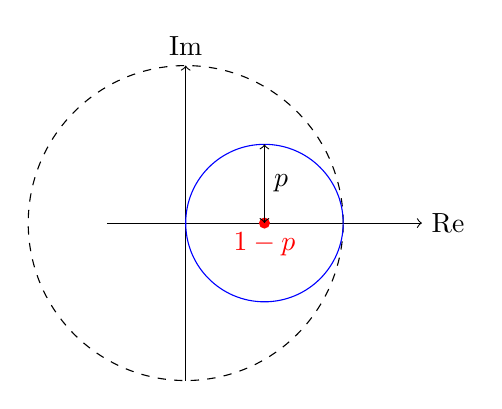
\begin{tikzpicture}[scale=2]
  % Parameters
  \def\p{0.5}

  % Axes
  \draw[->] (-0.5,0) -- (1.5,0) node[right] {Re};
  \draw[->] (0,-1) -- (0,1) node[above] {Im};

  % Unit circle
  \draw[dashed] (0,0) circle (1);

  % Circle representing xi
  \draw[blue] (1-\p,0) circle (\p);

  % Center point
  \fill[red] (1-\p,0) circle (1pt) node[below] {$1-p$};

  % Radius label
  \draw[<->] (1-\p,0) -- ++(0,\p) node[midway,right] {$p$};
\end{tikzpicture}

So the scheme is stable if \(\abs{\xi} \leq 1 \) if \(0 < p \leq 1\) or \(0 < a \frac{k}{h} \leq 1\).

What happens if we have \(a < 0\)? In this case the condition \(\abs{\xi} \leq 1 \) for all \( \beta \) is not satisfied.

\subparagraph{Forward Time, Central Space}

\[
  U_m^{n+1} = U_m^n - \frac{p}{2}\left( U_{m+1}^n - U_{m-1}^n \right)
\]

Then we get the stability condition:

\begin{align*}
  \xi       & = 1 - \frac{p}{2}\left( e^{i\beta h} - e^{-i\beta h} \right) = 1 - p\sin(\beta h) \\
  \abs{\xi} & = \sqrt{(1 - p\sin^2(\beta h))} = 1 - p\sin(\beta h) \leq 1
\end{align*}

\clearpage
\section{Forelesning 12 (Tirsdag11. februar 2025)}

\begin{definition}{Courant-Friedrichs-Lewy condition (CFL)}{cfl}
  The CFL condition is a necessary condition for the stability of a numerical scheme for solving PDEs.
  It states that the time step \(k\) must be chosen such that
  \[
    \abs{a} \frac{k}{h} \leq 1
  \]
  where \(a\) is the speed of the wave, \(k\) is the time step, and \(h\) is the spatial step.

  \[
    C = \frac{k}{h} \abs{a} \tag {Courant number}
  \]

\end{definition}

For the FTCS scheme, we have
\begin{align*}
  \frac{1}{k}\left( U_m^{n+1} - U_m^n \right) + \frac{a}{2h}\left( U_{m-1}^n - U_{m+1}^n \right) \\
  U_m^{n+1} = U_m^n - \frac{p}{2}\left( U_{m+1}^n - U_{m-1}^n \right) \quad p = a \frac{k}{h}
\end{align*}

\subparagraph{Von Neumann Stability Analysis}
\begin{align*}
  U_m^n = \xi^n e^{i\beta m} \\
  \xi = 1 - ip\sin(\beta h)  \\
  \abs{\xi} = \sqrt{1 - p^2\sin^2(\beta h)} \leq 1
\end{align*}

\subparagraph{Lax-Friedrichs Scheme}
\begin{align*}
  U_m^{n+1} = \frac{1}{2}\left( U_{m+1}^n + U_{m-1}^n \right) - \frac{p}{2}\left( U_{m+1}^n - U_{m-1}^n \right)
\end{align*}

\subparagraph{Von Neumann Stability Analysis}
\begin{align*}
  U_m^n = \xi^n e^{i\beta m}                                                                                            \\
  \xi = \frac{1}{2}\left( e^{i\beta h} + e^{-i\beta h} \right) - \frac{p}{2}\left( e^{i\beta h} - e^{-i\beta h} \right) \\
  \xi = \cos(\beta h) - ip\sin(\beta h)                                                                                 \\
  \abs{\xi}^2 = \cos^2(\beta h) + p^2\sin^2(\beta h)                                                                    \\
  \abs{\xi} = \sqrt{\left( \frac{1}{2} - \frac{p}{2}\sin(\beta h) \right)^2} \leq 1 \quad \text{if} \quad p \leq 1
\end{align*}

\begin{align*}
  \tau_m^n = -\frac{1}{2}\frac{h}{k}h \partial_x^2 u_m^n + O(k + h^2) \\
\end{align*}

The scheme is consistent of order 1 in time and 2 in space if \(h/k\) is constant.

Now we can rewrite the \textit{Lax-Friedrichs scheme} as
\[
  U_m^{n+1} = U_m^n - \frac{p}{2}\left( U_{m+1}^n - U_{m-1}^n \right) + \frac{1}{2}\left( U_{m+1}^n - 2U_m^n + U_{m-1}^n \right)
\]

This approximates:
\[
  \partial_t u = -a \partial_x u + \varepsilon \partial_x^2 u, \quad \varepsilon = \frac{h^2}{2k} \tag{Artificial diffusion}
\]

\subparagraph{Lax-Wendroff Scheme}
Evaluate the following at \((x,t)\):
\begin{align*}
  \begin{cases}
    u_t = -a u_x                   \\
    u_{tt} = -a u_{xt} = -a u_{tx} \\
    u_{tt} = a^2 u_{xx}
  \end{cases}                                                                                                                \\
  u(x, t + k) & = u + k u_t + \frac{1}{2}k^2 u_{tt} + O(k^3)                                                                                    \\
  u(x, t + k) & = u - a k u_x + \frac{1}{2}k^2 a^2 u_{xx} + O(k^3)                                                                              \\
  U_m^{n+1}   & = U_m^n - a \frac{k}{2h}\left( U_{m+1}^n - U_{m-1}^n \right) + \frac{a^2k^2}{2h^2}\left( U_{m+1}^n - 2U_m^n + U_{m-1}^n \right) \\
  \varepsilon = \frac{a^2k^2}{2h^2} \tag{Artificial diffusion}                                                                                  \\
  \tau_m^n    & = O(k^2 + h^2) \quad \text{Consistent of order 2}                                                                               \\
  \xi         & = 1 - ip\sin(\beta h) + p^2\left( \cos(\beta h) - 1 \right)                                                                     \\
  \abs{\xi} \leq 1 \quad \text{if} \quad p \leq 1
\end{align*}

We can prove that the Lax-Wendroff scheme is stable if \(p \leq 1\) if \(\frac{h^2}{2k} \leq \varepsilon \leq \frac{a^2k^2}{2}\).

\subparagraph{Wendroff Scheme}
Let \(u_t + a u_x = 0\), then we integrate the equation over the interval \([x_m, x_m + h]\) and \([t_n, t_n + k]\) and get

\begin{align*}
  \int_{t_n}^{t_n + k} \int_{x_m}^{x_m + h} \left( u_t + a u_x \right) \, dx \, dt = 0                                                         \\
  \int_{t_n}^{t_n + k} \int_{x_m}^{x_m + h} u_t \, dx \, dt = - a \int_{t_n}^{t_n + k} \int_{x_m}^{x_m + h} u_x \, dx \, dt                    \\
  \int_{x_m}^{x_m + h} \left( u(x, t_{n+1}) - u(x, t_n) \right) \, dx = -a \int_{t_n}^{t_n + k} \left( u(x_{m+1}, t) - u(x_m, t) \right) \, dt \\
\end{align*}

Using the trapezoidal rule:

\[
  \int_a^b f(x) \, dx \approx \frac{b-a}{2}\left( f(a) + f(b) \right)
\]

\begin{align*}
  \frac{h}{2}\left[u_{m+1}^{n+1}+u_m^{n+1}-u_{m+1}^n-u_m^n\right] =  -\frac{k}{2}\left[u_{m+1}^{n+1}+u_{m+1}^n-u_m^{n+1}-u_m^n\right] + \text{Error} \\
  U_m^{n+1} = U_m^n - \frac{a k}{2h}\left( U_{m+1}^n - U_{m-1}^n \right) + \frac{a^2 k^2}{2h^2}\left( U_{m+1}^n - 2U_m^n + U_{m-1}^n \right)
\end{align*}


\begin{align*}
  U_m^{n+1}     & =
  \begin{cases}
    -p \nabla_h U_m^n                                    & \text{FTBS (Upwind)}  \\
    -p\mu_k \delta_h U_m^n + \frac{1}{2}\delta_h^2 U_m^n & \text{Lax-Friedrichs} \\
    -p\mu_k \delta_h U_m^n + \frac{1}{2}\delta_h^2 U_m^n & \text{Lax-Wendroff}
  \end{cases} \\
  U_{m+1}^{n+1} & = U_m^n + \frac{1-p}{1+p}\left(U_{m+1}^n - U_m^{n}\right)
\end{align*}


The \textit{courant number} is defined as

\[
  C = \frac{a k}{h}
\]

We can also get \textbf{Dissipation} and \textbf{Dispersion}.

Let \(u_t = \mathcal{L}_t u\), with \(u(x) = f(x)\).
The idea is to find the solution of the PDE on the form \(u(x,t) = e^{i\omega t}e^{i\beta x}\) and then plug it into the PDE and solve for \(\omega= \omega(\beta)\), where \(\beta\) is the frequency (mode).

For the complete problem we get:

\begin{align*}
  u(x,t) =
  \begin{cases}
    \sum_{n=-\infty}^{+\infty} C_n e^{i\omega(\beta_n)t}e^{i\beta_n x}          & \text{if} \quad f \quad \text{is periodic} \\
    \int_{-\infty}^{+\infty} C(\beta) e^{i\omega(\beta)t}e^{i\beta x} \, d\beta & \text{otherwise}
  \end{cases}
\end{align*}

\begin{example}{}{}
  \[
    u_t + a u_x = 0, \quad u(x,0) = f(x)
  \]

  \begin{align*}
    u(x,t)        & = f(x-at)                                         \\
    \omega(\beta) & = -a\beta                                         \\
    u(x,t)        & = e^{i\beta(x - at)} = e^{i\beta x}e^{-i\omega t}
  \end{align*}

\end{example}

\begin{example}{}{}
  \[
    u_t = \mu u_{xx}, \quad \mu > 0, \quad \text{Dissipation}
  \]

  \begin{align*}
    i\omega = -\mu \beta^2 \implies \omega = -i\mu \beta^2 \\
    u(x,t) = e^{-\mu \beta^2 t}e^{i\beta x}
  \end{align*}

\end{example}

\begin{example}{}{}
  \[
    u_t + a u_{xxx} = 0, \quad \text{No dissipation} \quad \text{Dispersion}
  \]

  \begin{align*}
    i\omega - i\beta^3 a = 0 \implies \omega = \beta^3 a \\
    u(x,t) = e^{i\beta x}e^{i\beta^3 a t}
  \end{align*}

  With phase velocity \(v_p = a \beta^2\), which is the speed of the wave.

  This is a dispersive wave equation.
\end{example}


\begin{definition}{Dissipation}{}
  Dissipation is the process of converting mechanical energy into heat. It is a damping effect.

  \begin{itemize}
    \item No modes increase by time.
    \item At least one mode decreases by time.
  \end{itemize}

  \begin{align*}
    \Im(\omega(\beta)) \geq 0 \\
    \text{At least one mode decreases by time} \implies \Im(\omega(\beta)) < 0
  \end{align*}
\end{definition}

\begin{definition}{Dispersion}{}
  Dispersion is the spreading of waves as they propagate. It is a spreading effect.

  \begin{itemize}
    \item The phase velocity \(v_p\) depends on the frequency \(\beta\).
  \end{itemize}
  \[
    \Re(\omega(\beta)) \neq C \beta, \quad C = \text{constant}
  \]

\end{definition}

\begin{example}{FTBS}{}
  Let \(a > 0\) and \(p = a \frac{k}{h} \leq 1\) with:

  \[
    U_m^{n+1} = U_m^n - p(U_{m+1}^n - U_m^n)
  \]

  \textbf{Stability:}
  \begin{align*}
    \xi = 1 - p(1 - e^{-i\beta h}) = (1 - p) + pe^{-i\beta h}                                                                                                                        \\
    \abs{\xi} = \sqrt{1 + 4p(1-p)\sin^2\frac{\beta h}{2}} = 1 - \frac{1}{2}p(1-p)\beta^2 h^2 + O((\beta h)^4)                                                                        \\
    \Phi = \arctan\left(\frac{-p\sin(\beta h)}{1-p(1-\cos(\beta h))}\right) = -p (\beta h)\left(1 - (\frac{1}{6} - \frac{1}{2}p + \frac{1}{3}p^2)(\beta h)^2 + O((\beta h)^4)\right) \\
    p (\beta h) = \frac{a k}{h} \beta h = a k \beta = C \beta
  \end{align*}

\end{example}
\section{Forelesning 13 (Mandag 17. februar 2025)}

\subsection{Hyperbolic Conservation Laws}

\paragraph{Euler's Equations in Gas Dynamics}
Consider the 1D Euler system:
\begin{align*}
  \rho_t + (\rho u)_x           & = 0, \\
  (\rho u)_t + (\rho u^2 + p)_x & = 0, \\
  E_t + \bigl(u(E + p)\bigr)_x  & = 0,
\end{align*}
where
\begin{align*}
  \rho = \rho(x,t) \; \text{(density)},\quad
  u = u(x,t) \; \text{(velocity)},\quad
  p = p(x,t) \; \text{(pressure)},\quad
  E = E(x,t) \; \text{(total energy)}.
\end{align*}

\begin{figure}[H]
  \centering
  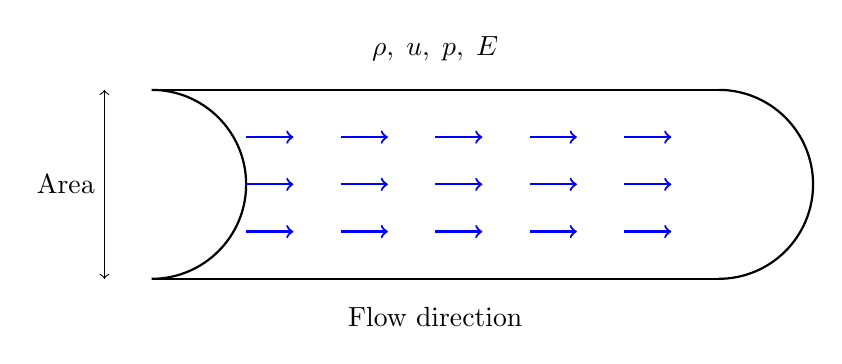
\begin{tikzpicture}[scale=1.2]
    % Draw the tube
    \draw[thick] (0,1) -- (6,1);
    \draw[thick] (0,-1) -- (6,-1);

    % Cross section at left
    \draw[thick] (0,-1) arc (-90:90:1);
    % Cross section at right
    \draw[thick] (6,-1) arc (-90:90:1);

    % Flow arrows (blue)
    \foreach \x in {1,2,3,4,5}
      {
        \draw[->,thick,blue] (\x,-0.5) -- (\x+0.5,-0.5);
        \draw[->,thick,blue] (\x,0) -- (\x+0.5,0);
        \draw[->,thick,blue] (\x,0.5) -- (\x+0.5,0.5);
      }

    % Labels
    \node[above] at (3,1.2) {\(\rho,\;u,\;p,\;E\)};
    \node[below] at (3,-1.2) {Flow direction};

    % Cross section labels
    \draw[<->] (-0.5,-1) -- (-0.5,1) node[midway,left] {Area};
  \end{tikzpicture}
\end{figure}

\begin{itemize}
  \item \(\rho(x,t)\) is the density of the gas.
  \item \(u(x,t)\) is the velocity of the gas.
  \item \(\rho\,u\) is the mass flux (mass per unit time).
  \item The mass in the interval \([a,b]\) at time \(t\) is
        \[
          m(t) \;=\; \int_a^b \rho(x,t)\,\mathrm{d}x
        \]
  \item Differentiating \(m(t)\) in time and using the Divergence Theorem (or the Fundamental Theorem of Calculus) leads to
        \begin{align*}
          \frac{d}{dt}\int_{a}^{b} \rho(x,t)\,dx
                                   & = \int_a^b \rho_t(x,t)\,\mathrm{d}x              \\
                                   & = \rho(a,t)\,u(a,t) \;-\; \rho(b,t)\,u(b,t)      \\
                                   & = - \int_a^b \bigl(\rho\,u\bigr)_x \,\mathrm{d}x
          \\
          \implies \quad
          \rho_t \;+\; (\rho\,u)_x & = 0
          \quad\tag{Conservation of mass}.
        \end{align*}
  \item Similarly, one obtains
        \[
          (\rho\,u)_t + (\rho\,u^2 + p)_x = 0
          \quad\tag{Conservation of momentum},
        \]
        and
        \[
          E_t + \bigl(u(E + p)\bigr)_x = 0
          \quad\tag{Conservation of energy}.
        \]
  \item Here \(p = p(\rho,\rho u,E)\) and \(E = E(\rho,\rho u,p)\) are related by the equation of state (e.g., an ideal gas law).
  \item \textbf{Vector form}:
        \[
          \begin{bmatrix}
            \rho   \\
            \rho u \\
            E
          \end{bmatrix}_t
          +
          \begin{bmatrix}
            \rho u       \\
            \rho u^2 + p \\
            u(E + p)
          \end{bmatrix}_x
          = 0,
          \quad
          p = p(\rho,\rho u,E),\quad
          E = E(\rho,\rho u,p).
        \]
\end{itemize}

\paragraph{General Hyperbolic Conservation Law}
In general, a (1D) hyperbolic conservation law has the form
\[
  \mathbf{u}_t \;+\; \bigl(\mathbf{f}(\mathbf{u})\bigr)_x \;=\; 0,
\]
where
\[
  \mathbf{u}
  =
  \begin{bmatrix}
    u_1    \\
    u_2    \\
    \vdots \\
    u_n
  \end{bmatrix}
  \quad\text{is the vector of conserved variables,}
  \quad
  \mathbf{f}(\mathbf{u})
  =
  \begin{bmatrix}
    f_1(\mathbf{u}) \\
    f_2(\mathbf{u}) \\
    \vdots          \\
    f_n(\mathbf{u})
  \end{bmatrix}
  \quad\text{is the flux function.}
\]
The Jacobian matrix \(\mathbf{f}'(\mathbf{u})\) has real eigenvalues and is diagonalizable in a hyperbolic system.

\smallskip

\textbf{From now on}, we often focus on a \emph{scalar} conservation law:
\[
  u_t + \bigl(f(u)\bigr)_x = 0.
\]

\paragraph{Burgers' Equation (scalar prototype)}
\[
  u_t + \left(\tfrac12\,u^2\right)_x = 0,
  \quad
  \text{or equivalently}
  \quad
  u_t + u\,u_x = 0.
\]

\smallskip
Let \(m(t) = \int_a^b u(x,t)\,\mathrm{d}x\). By an analogous argument, the flux boundary terms appear:
\[
  \frac{d\,m}{dt}
  \;=\;
  \int_a^b u_t(x,t)\,\mathrm{d}x
  \;=\;
  f(a,t)\;-\;f(b,t),
\]
which again expresses conservation of mass (or the conserved quantity).

\paragraph{Conservative Schemes (Finite Difference Discretization)}
Consider a one-step scheme of the form
\[
  U_m^{n+1}
  \;=\;
  U_m^n
  \;-\;
  p\,\Bigl[F\bigl(U_m^n,\,U_{m+1}^n\bigr) \;-\; F\bigl(U_{m-1}^n,\,U_m^n\bigr)\Bigr],
\]
where \(p\) is the CFL-like factor \(\frac{k}{h}\) (time-step over space-step), and \(F(\cdot,\cdot)\) is called the \emph{numerical flux} function.

\begin{figure}[H]
  \centering
  \begin{tikzpicture}[scale=1.5]
    % Axes
    \draw[->] (-1,0) -- (3,0) node[right] {$x$};
    \draw[->] (0,-1) -- (0,3) node[above] {$t$};

    % Points
    \filldraw[black] (0,0) circle (1.5pt) node[below left] {$U_{m-1}^n$};
    \filldraw[black] (1,0) circle (1.5pt) node[below] {$U_{m}^n$};
    \filldraw[black] (2,0) circle (1.5pt) node[below right] {$U_{m+1}^n$};
    \filldraw[black] (1,1) circle (1.5pt) node[above] {$U_{m}^{n+1}$};

    % Arrows showing dependencies
    \draw[->,thick,blue] (0,0) -- (1,0);
    \draw[->,thick,blue] (1,0) -- (1,1);
    \draw[->,thick,blue] (2,0) -- (1,0);

    % Dashed lines for cell boundaries
    \draw[dashed,red] (0.5,-0.25) -- (0.5,0.75);
    \draw[dashed,red] (1.5,-0.25) -- (1.5,0.75);

    % Flux indicators
    \node[red, left] at (0.5,0.25) {$F(U_{m-1}^n,\,U_m^n)$};
    \node[red, right] at (1.5,0.25) {$F(U_{m}^n,\,U_{m+1}^n)$};
  \end{tikzpicture}
  \caption{Conservative scheme stencil with fluxes.}
\end{figure}

\noindent
\textbf{Why is this conservative?}

If we define
\[
  \mathbf{U}^n
  \;=\;
  \begin{bmatrix}
    U_1^n  \\
    U_2^n  \\
    \vdots \\
    U_M^n
  \end{bmatrix},
\]
then we can interpret the sum of discrete values as approximating an integral (for example, via the trapezoidal rule or midpoint rule). One shows that the scheme
\[
  U_m^{n+1}
  \;=\;
  U_m^n
  \;-\;
  p\,\Bigl[
  F(U_m^n,\,U_{m+1}^n) \;-\; F(U_{m-1}^n,\,U_m^n)
  \Bigr]
\]
implies the total sum
\(\sum_{m=1}^{M-1} U_m^n\) changes by discrete boundary terms only, analogous to the continuum case
\(\int_a^b u_t\,dx = f(a,t) - f(b,t)\). This ensures conservation in discrete form.

\subsection{Example: Transport Equation}

Consider the linear transport (advection) equation
\[
  u_t + a\,u_x = 0,
  \quad a>0,
  \quad
  \text{with } p := a\,\frac{k}{h}.
\]
A classic upwind (FTBS) scheme is:
\[
  U_m^{n+1}
  \;=\;
  U_m^n - p\Bigl(U_m^n - U_{m-1}^n\Bigr)
  \;=\;
  U_m^n - p\Bigl[f(U_m^n) - f(U_{m-1}^n)\Bigr],
\]
where \(f(u) = a\,u\). This scheme is conservative with the numerical flux
\[
  F\bigl(U_m^n,\,U_{m+1}^n\bigr) = a\,U_m^n = f(U_m^n).
\]

\paragraph{Burger's Equation}
\[
  u_t + \frac{1}{2}\bigl(u^2\bigr)_x = 0
  \quad\Leftrightarrow\quad
  u_t + u\,u_x = 0.
\]

\subsection{Lax--Friedrichs Scheme}
A well-known conservative scheme is the Lax--Friedrichs method:
\[
  U_m^{n+1}
  \;=\;
  \frac12\,\bigl(U_{m+1}^n + U_{m-1}^n\bigr)
  \;-\;
  \frac{p}{2}\,\Bigl(f(U_{m+1}^n) - f(U_{m-1}^n)\Bigr).
\]
Its numerical flux is often written as
\[
  F\bigl(U_m^n,\,U_{m+1}^n\bigr)
  \;=\;
  \frac12\Bigl(f(U_m^n)+f(U_{m+1}^n)\Bigr)
  \;-\;
  \frac{\alpha}{2}\,\bigl(U_{m+1}^n - U_m^n\bigr),
\]
where \(\alpha\) is some stability-related term (often chosen \(\alpha = \max |f'(u)|\) over relevant states). This guarantees stability and conservation.

\subsection{Lax--Wendroff Scheme}
For a conservation law \(u_t + (f(u))_x = 0\) with \(a(u) = f'(u)\), the Lax--Wendroff update reads:
\[
  U_m^{n+1}
  =
  U_m^n
  \;-\;
  \frac{p}{2}\Bigl[f(U_{m+1}^n)-f(U_{m-1}^n)\Bigr]
  \;+\;
  \frac{p^2}{2}\Bigl[
    a_{m+\tfrac12}\,\bigl(U_{m+1}^n - U_m^n\bigr)
    \;-\;
    a_{m-\tfrac12}\,\bigl(U_m^n - U_{m-1}^n\bigr)
    \Bigr],
\]
where
\[
  a_{m\pm\tfrac12}
  =
  \begin{cases}
    \tfrac12\bigl(a(U_m^n)+a(U_{m\pm1}^n)\bigr),            & \text{(Lax--Friedrichs approach)}, \\[6pt]
    a\!\Bigl(\tfrac12\bigl(U_m^n + U_{m\pm1}^n\bigr)\Bigr), & \text{(Lax--Wendroff approach)}.
  \end{cases}
\]
Here, \(a(u) = \frac{d}{du}f(u)\). The difference between the two choices mainly lies in how you approximate \(a(u)\) at the half-integer points.
\section{Forelesning 14 (Tirsdag 18. februar 2025)}
\subsection{Elliptic PDEs}\footnote{Section 6 in B.O.}

\begin{figure}[H]
  \centering
  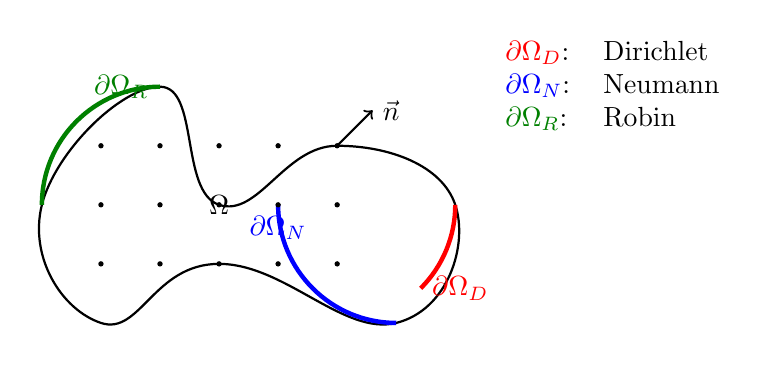
\begin{tikzpicture}[scale=1.5]
    % Draw the main Omega domain with a "squiggly" border
    \draw[thick] plot [smooth cycle, tension=0.8] coordinates {
        (0,0) (1,0.5) (2,0) (1.5,-1) (0,-0.5) (-1,-1) (-1.5,0) (-0.5,1)
      };

    % Add colored arcs for different boundary segments
    \draw[red, ultra thick] (2,0) arc (0:-45:1) node[right] {$\partial\Omega_D$};
    \draw[blue, ultra thick] (1.5,-1) arc (-90:-180:1) node[below] {$\partial\Omega_N$};
    \draw[green!50!black, ultra thick] (-1.5,0) arc (180:90:1) node[left] {$\partial\Omega_R$};

    % Label the domain
    \node at (0,0) {$\Omega$};

    % Normal vector example
    \draw[->, thick] (1,0.5) -- (1.3,0.8) node[right] {$\vec{n}$};

    % Some discrete grid points as an illustration
    \foreach \x in {-1,-0.5,0,0.5,1}
    \foreach \y in {-0.5,0,0.5}
    \filldraw[black] (\x,\y) circle (0.5pt);

    % Boundary legend
    \node[right] at (2.2,1) {
      \begin{tabular}{ll}
        \textcolor{red}{$\partial\Omega_D$}:            & Dirichlet \\
        \textcolor{blue}{$\partial\Omega_N$}:           & Neumann   \\
        \textcolor{green!50!black}{$\partial\Omega_R$}: & Robin
      \end{tabular}
    };
  \end{tikzpicture}
\end{figure}

\paragraph{Boundary Conditions}
\begin{itemize}
  \item \textbf{Dirichlet:} \(u = g\) on \(\partial\Omega_D\).
  \item \textbf{Neumann:} \(\frac{\partial u}{\partial \vec{n}} = \vec{n}\cdot\nabla u = g\) on \(\partial\Omega_N\).
  \item \textbf{Robin (Mixed):} \(\alpha\,u + \beta\,\frac{\partial u}{\partial n} = g\) on \(\partial\Omega_R\).
\end{itemize}

\[
  \partial \Omega \;=\;
  \overline{\partial \Omega_D \;\cup\; \partial\Omega_N \;\cup\; \partial\Omega_R}.
\]

\begin{enumerate}
  \item Find a finite difference scheme (FDS) for the model problem.
  \item Implement and test the method.
  \item Perform an error analysis.
  \item Discuss how to handle more complicated boundaries and irregular grids.
\end{enumerate}

\subsubsection{Model Problem (Poisson Equation)}
\[
  \begin{cases}
    u_{xx} + u_{yy} = f(x,y), & \text{in } \Omega = (0,1) \times (0,1),                               \\[6pt]
    u = g,                    & \text{on } \partial \Omega_D \;\; (x=0,\,x=1,\,y=0,\,\text{or}\,y=1).
  \end{cases}
\]

\begin{enumerate}
  \item \emph{FDS:} Discretize the domain and boundary:
        \[
          \Omega_h = \{(x_i,y_j)\,|\,x_i = i\,h,\;y_j = j\,h,\;i,j=0,1,\ldots,N\},
        \]
        \[
          \partial\Omega_{D,h} = \{(x_i,y_j)\,\in\,\Omega_h \;\mid\; i=0\text{ or }i=N\text{ or }j=0\text{ or }j=N\},
        \]
        \[
          \mathring{\Omega}_h = \Omega_h \setminus \partial\Omega_{D,h}.
        \]

  \item \emph{Test:} Implement the method with central finite differences. For example,
        \[
          u_{xx}(x_i,y_j) \;\approx\; \frac{u_{i+1,j} - 2\,u_{i,j} + u_{i-1,j}}{h^2}
          \;+\;\frac{h^2}{6}\,\partial_x^4u(x_i,y_j),
        \]
        and similarly for \(u_{yy}\). Then
        \[
          \frac{1}{h^2}\bigl(U_{i+1,j} + U_{i,j+1} - 4\,U_{i,j} + U_{i-1,j} + U_{i,j-1}\bigr)
          \;=\; f_{i,j}.
        \]

  \item \emph{Computational Stencil:}
        Let \(P=(x_i,y_j)\), \(E=(x_{i+1},y_j)\), \(N=(x_i,y_{j+1})\), \(W=(x_{i-1},y_j)\), and \(S=(x_i,y_{j-1})\). Then
        \[
          U_{i,j}
          \;=\;
          \frac{1}{4}\Bigl(U_{i+1,j} \;+\; U_{i,j+1} \;+\; U_{i-1,j} \;+\; U_{i,j-1}\Bigr)
          \;-\;
          \frac{h^2}{4}\,f_{i,j}.
        \]
        Or equivalently:
        \[
          U_N + U_E + U_W + U_S \;-\;4\,U_P = h^2\,f_P,
          \quad P \in \mathring{\Omega}_h.
        \]

  \item \emph{Error Analysis:} Estimate \(\|u - U\|\) in an appropriate norm. The standard result shows an \(\mathcal{O}(h^2)\) error for sufficiently smooth \(u\).
\end{enumerate}

\begin{definition}{Natural Ordering}{}
  \begin{figure}[H]
    \centering
    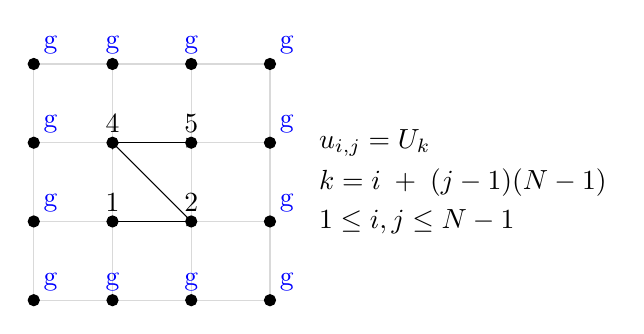
\begin{tikzpicture}[scale=1]
      % Grid
      \draw[step=1cm,gray!30] (0,0) grid (3,3);

      % Node points
      \foreach \x in {0,1,2,3}
      \foreach \y in {0,1,2,3} {
          \filldraw[black] (\x,\y) circle (2pt);
        }

      % Example labeling for natural ordering inside
      \node[above] at (1,1) {1};
      \node[above] at (2,1) {2};
      \node[above] at (1,2) {4};
      \node[above] at (2,2) {5};

      % Boundary points labeled g
      \foreach \x in {0,3}
      \foreach \y in {0,1,2,3}
      \node[blue, above right] at (\x,\y) {g};

      \foreach \x in {1,2}
      \foreach \y in {0,3}
      \node[blue, above] at (\x,\y) {g};

      % Arrows for ordering
      \draw[->] (1,1) -- (2,1);
      \draw[->] (2,1) -- (1,2);
      \draw[->] (1,2) -- (2,2);

      % Equations on right
      \node[right] at (3.5,2) {$u_{i,j} = U_k$};
      \node[right] at (3.5,1.5) {$k = i \;+\;(j-1)(N-1)$};
      \node[right] at (3.5,1) {$1 \le i,j \le N-1$};
    \end{tikzpicture}
    \caption{Natural ordering of interior grid points.}
  \end{figure}

  In matrix form, the 5-point stencil leads to:
  \[
    \frac{1}{h^2}
    \begin{bmatrix}
      -4     & 1      & 0      & \cdots & 0      & 1      & 0      & \cdots & 0      \\
      1      & -4     & 1      & \cdots & 0      & 0      & 1      & \cdots & 0      \\
      0      & 1      & -4     & \cdots & 0      & 0      & 0      & \cdots & 0      \\
      \vdots & \vdots & \vdots & \ddots & \vdots & \vdots & \vdots & \ddots & \vdots \\
      1      & 0      & 0      & \cdots & -4     & 1      & 0      & \cdots & 0      \\
      0      & 1      & 0      & \cdots & 1      & -4     & 1      & \cdots & 0      \\
      \vdots & \vdots & \vdots & \ddots & \vdots & \vdots & \vdots & \ddots & \vdots \\
      0      & 0      & 0      & \cdots & 0      & 1      & 0      & \cdots & -4
    \end{bmatrix}
    \begin{bmatrix}
      U_{1,1} \\
      U_{2,1} \\
      \vdots  \\
      U_{1,2} \\
      U_{2,2} \\
      \vdots  \\
      U_{N-1,N-1}
    \end{bmatrix}
    =
    \begin{bmatrix}
      f_{1,1} - \frac{1}{h^2}(g_W + g_S) \\
      f_{2,1} - \frac{1}{h^2}\,g_S       \\
      \vdots                             \\
      f_{1,2} - \frac{1}{h^2}\,g_W       \\
      f_{2,2}                            \\
      \vdots                             \\
      f_{N-1,N-1} - \frac{1}{h^2}(g_E + g_N)
    \end{bmatrix}.
  \]

\end{definition}

\begin{figure}[H]
  \centering
  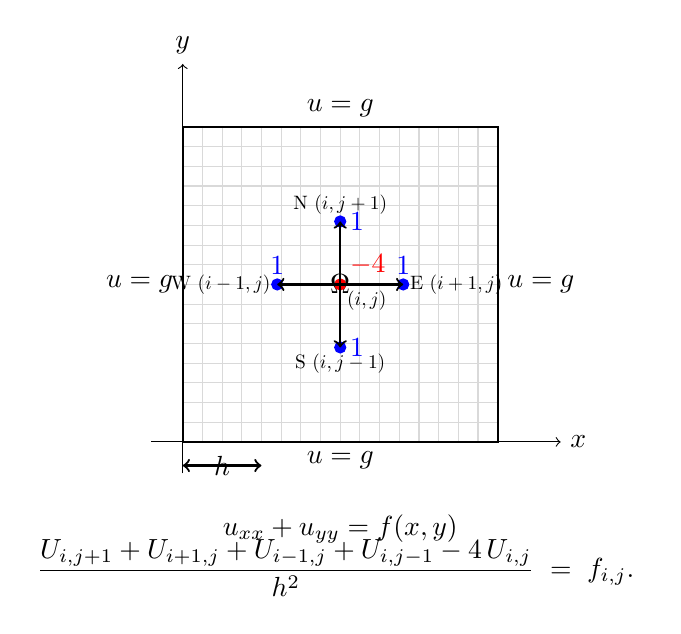
\begin{tikzpicture}[scale=1]
    % Grid
    \draw[step=0.25,gray!30] (0,0) grid (4,4);

    % Domain boundary
    \draw[thick] (0,0) rectangle (4,4);

    % Axes
    \draw[->] (-0.4,0) -- (4.8,0) node[right] {$x$};
    \draw[->] (0,-0.4) -- (0,4.8) node[above] {$y$};

    % Label domain
    \node at (2,2) {$\Omega$};

    % Boundary conditions
    \node[left] at (0,2) {$u=g$};
    \node[right] at (4,2) {$u=g$};
    \node[below] at (2,0) {$u=g$};
    \node[above] at (2,4) {$u=g$};

    % Stencil points
    \filldraw[red] (2,2) circle (2pt) node[below right,black,scale=0.7] {$(i,j)$};
    \filldraw[blue] (2.8,2) circle (2pt) node[right,black,scale=0.7] {E $(i+1,j)$};
    \filldraw[blue] (2,2.8) circle (2pt) node[above,black,scale=0.7] {N $(i,j+1)$};
    \filldraw[blue] (1.2,2) circle (2pt) node[left,black,scale=0.7] {W $(i-1,j)$};
    \filldraw[blue] (2,1.2) circle (2pt) node[below,black,scale=0.7] {S $(i,j-1)$};

    % Arrows
    \draw[->,thick] (2,2) -- (2.8,2);
    \draw[->,thick] (2,2) -- (2,2.8);
    \draw[->,thick] (2,2) -- (1.2,2);
    \draw[->,thick] (2,2) -- (2,1.2);

    % Equation labels
    \node[below] at (2,-0.8) {$u_{xx} + u_{yy} = f(x,y)$};

    % Coefficients in the stencil
    \node[red] at (2,2) [above right] {$-4$};
    \node[blue] at (2.8,2) [above] {$1$};
    \node[blue] at (2,2.8) [right] {$1$};
    \node[blue] at (1.2,2) [above] {$1$};
    \node[blue] at (2,1.2) [right] {$1$};

    % Mesh size
    \draw[<->, thick] (0,-0.3) -- (1,-0.3);
    \node at (0.5,-0.3) {$h$};

    % Discrete formula
    \node[align=center] at (2,-1.6) {
    $\displaystyle \frac{U_{i,j+1} + U_{i+1,j} + U_{i-1,j} + U_{i,j-1} - 4\,U_{i,j}}{h^2} \;=\; f_{i,j}.$
    };
  \end{tikzpicture}
\end{figure}

\paragraph{Matrix Form}
Define
\[
  \mathbf{A} \;=\;
  \operatorname{blocktridiag}\bigl(B,\;I,\;I\bigr)
  \;\in\;\mathbb{R}^{(M-1)^2 \times (M-1)^2},
\]
where
\[
  B \;=\;
  \operatorname{tridiag}(1,\,-4,\,1)
  \;\in\;\mathbb{R}^{(M-1)\times(M-1)}.
\]
Hence, \(\mathbf{A}\) is large but \emph{sparse} and \emph{banded}. For example, if \(M=100\), then \(\mathbf{A}\in \mathbb{R}^{9801\times 9801}\). Efficient iterative solvers (e.g., Gauss--Seidel, CG, GMRES) can exploit this sparsity.

\begin{definition}{5-Point Formula}{5_pnt_formula}
  The \emph{5-point formula} for discretizing the Poisson equation
  \[
    u_{xx} + u_{yy} = f
  \]
  is
  \[
    U_{i,j}
    \;=\;
    \frac{1}{4}
    \bigl(U_{i+1,j} + U_{i,j+1} + U_{i-1,j} + U_{i,j-1}\bigr)
    \;-\;
    \frac{h^2}{4}\,f_{i,j}.
  \]
  It approximates each interior grid point \(U_{i,j}\) using its four neighbors and has a local truncation error of \(\mathcal{O}(h^2)\).
\end{definition}
\section{Forelesning 15 (Mandag 24. februar 2025)}
\subsection{Poisson's Equation on the Unit Square with a Regular Grid}

Let \(\Omega = (0,1)\times(0,1)\). We consider the boundary \(\partial\Omega\) to be the edges of the unit square. Define the operator \(\mathcal{L}u = \Delta u = u_{xx} + u_{yy}\), and assume
\[
  \begin{cases}
    \mathcal{L}u = f & \text{in } \Omega,           \\
    u = g            & \text{on } \partial\Omega_D.
  \end{cases}
\]

\begin{center}
  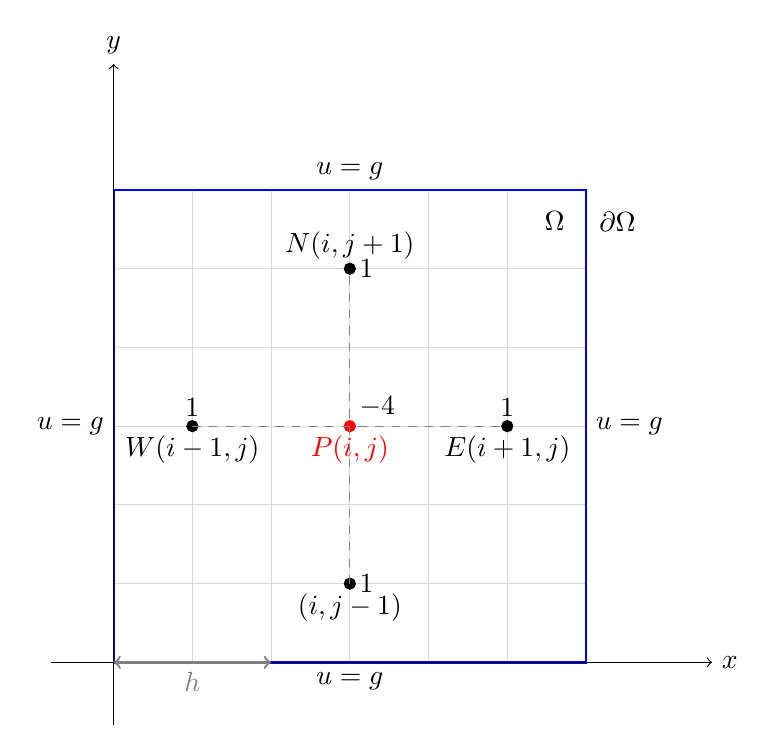
\begin{tikzpicture}[scale=2]
    % Grid 
    \draw[step=0.5cm,gray!30] (0,0) grid (3,3);

    % Domain (blue boundary for the unit square)
    \draw[thick,blue] (0,0) rectangle (3,3);

    % Axes
    \draw[->] (-0.4,0) -- (3.8,0) node[right] {$x$};
    \draw[->] (0,-0.4) -- (0,3.8) node[above] {$y$};

    % Label domain
    \node at (2.8,2.8) {$\Omega$};
    \node at (3.2,2.8) {$\partial\Omega$};

    % Label boundary conditions
    \node[left]  at (0,1.5) {$u=g$};
    \node[right] at (3,1.5) {$u=g$};
    \node[below] at (1.5,0) {$u=g$};
    \node[above] at (1.5,3) {$u=g$};

    % Center point and neighbors (P = point, N = north, S = south, E = east, W = west)
    \filldraw[red]  (1.5,1.5) circle (1pt) node[below] {$P(i,j)$};
    \filldraw[black] (2.5,1.5) circle (1pt) node[below]  {$E(i+1,j)$};
    \filldraw[black] (1.5,2.5) circle (1pt) node[above] {$N(i,j+1)$};
    \filldraw[black] (0.5,1.5) circle (1pt) node[below]  {$W(i-1,j)$};
    \filldraw[black] (1.5,0.5) circle (1pt) node[below] {$(i,j-1)$};

    % Connect points with dashed lines
    \draw[gray,dashed] (0.5,1.5) -- (2.5,1.5);
    \draw[gray,dashed] (1.5,0.5) -- (1.5,2.5);

    % Coefficient labels
    \node[black]  at (1.5,1.5) [above right] {$-4$};
    \node[black] at (2.5,1.5) [above]  {$1$};
    \node[black] at (1.5,2.5) [right]  {$1$};
    \node[black] at (0.5,1.5) [above]  {$1$};
    \node[black] at (1.5,0.5) [right]  {$1$};

    % Mesh size label
    \draw[<->, thick, gray] (0,0) -- (1,0) node[midway,below] {$h$};

  \end{tikzpicture}
\end{center}

\paragraph{5-Point Formula}
A common finite-difference approximation for \(u_{xx} + u_{yy}\) on a uniform grid (spacing \(h\)) is:
\[
  \Delta u \;\approx\; \frac{1}{h^2}\bigl(u_{i+1,j} + u_{i,j+1} + u_{i-1,j} + u_{i,j-1} - 4u_{i,j}\bigr).
\]

\paragraph{Error Analysis}
We want to find an upper bound for the error
\[
  e_{i,j} \;=\; u_{i,j} - U_{i,j},
\]
where \(U_{i,j}\) denotes the discrete solution. Typically, we can show
\[
  |e_{i,j}| \;\le\; C_1\,h^2 \;+\; C_2\,h^4,
  \quad
  \text{for interior points } (i,j) \in \mathring{\Omega}_h.
\]

\subparagraph{Local Truncation Error}
Define the local truncation error by
\[
  \tau_p \;=\; \mathcal{L}_h\,u_p \;-\; f_p,
\]
where \(\mathcal{L}_h\) is the discrete operator applied to the \emph{exact} solution \(u\). For interior grid points \(p\in \mathring{\Omega}_h\), we would like
\[
  \mathcal{L}_h\,u_p \;=\; f_p.
\]
On the boundary, \(\tau_p\) might be nonzero if we enforce boundary conditions in a particular way. We will use the discrete maximum principle to show that the global error is controlled by the local truncation error.

\subparagraph{Maximum Principle (Continuous)}
Let \(\Omega \subset \mathbb{R}^2\) be open and connected, and let \(v\) be a sufficiently smooth function on \(\overline{\Omega}\). Suppose \(\mathcal{L}u = u_{xx} + u_{yy}\).

\begin{itemize}
  \item If \(\mathcal{L}u \ge 0\) in \(\Omega\) and \(u = v\) on \(\partial\Omega\), then \(v \le \max_{\partial\Omega} v\).
  \item If \(\mathcal{L}u \le 0\) in \(\Omega\) and \(u = v\) on \(\partial\Omega\), then \(v \ge \min_{\partial\Omega} v\).
  \item If \(\mathcal{L}u = 0\) in \(\Omega\) and \(u = v\) on \(\partial\Omega\), then both the minimum and maximum of \(v\) are attained on the boundary.
\end{itemize}

\paragraph{Discrete Maximum Principle (5-Point Formula)}
Let \(\{v_p\}_{p \in \Omega_h}\) be values at the grid points, and define the discrete operator
\[
  \mathcal{L}_h\,v_p
  \;=\;
  \frac{1}{h^2}\bigl(v_E + v_N + v_W + v_S - 4\,v_P\bigr),
\]
where \(E, N, W, S\) denote the east, north, west, and south neighbors of \(p\), respectively.

\begin{itemize}
  \item If \(\mathcal{L}_h\,v_p \;\ge\; 0\) for all interior points \(p \in \Omega_h\), then for each interior point \(P\),
        \[
          v_P \;\le\; \max_{R \in \partial\Omega_h} v_R.
        \]
  \item If \(\mathcal{L}_h\,v_p \;\le\; 0\) for all interior points \(p \in \Omega_h\), then for each interior point \(P\),
        \[
          v_P \;\ge\; \min_{R \in \partial\Omega_h} v_R.
        \]
\end{itemize}

\begin{proof}[Proof by contradiction]
  Suppose \(\mathcal{L}_h\,v_p \ge 0\) in \(\Omega_h\). Assume there exists an interior point \(p^\star\) such that
  \[
    v_{p^\star} \;=\; \max_{p \in \overline{\Omega}_h} v_p.
  \]
  Then \(v_{p^\star} \ge v_{E^\star}, v_{N^\star}, v_{W^\star}, v_{S^\star}\). From
  \[
    \mathcal{L}_h v_{p^\star} \;=\; \frac{1}{h^2}\Bigl(v_{E^\star} + v_{N^\star} + v_{W^\star} + v_{S^\star} - 4\,v_{p^\star}\Bigr) \;\ge\; 0,
  \]
  we get
  \[
    4\,v_{p^\star} \;\le\; v_{E^\star} + v_{N^\star} + v_{W^\star} + v_{S^\star} \;\le\; 4\,v_{p^\star},
  \]
  which forces
  \[
    v_{p^\star} \;=\; v_{E^\star} \;=\; v_{N^\star} \;=\; v_{W^\star} \;=\; v_{S^\star}.
  \]
  Repeating this argument outward toward the boundary shows that \(v\) is constant or attains its maximum on the boundary. Hence
  \[
    \max_{p \in \overline{\Omega}_h} v_p \;=\; \max_{R \in \partial\Omega_h} v_R.
  \]
  An analogous argument applies for \(\mathcal{L}_h\,v_p \le 0\).
\end{proof}

\paragraph{Local Truncation Error (Detailed)}
Let
\[
  \tau_p
  \;=\;
  \mathcal{L}_h\,u_p - f_p
  \;=\;
  \mathcal{L}_h\,u_p \;-\; \mathcal{L}u_p.
\]
For \(\mathcal{L}_h\) given by
\[
  \mathcal{L}_h\,U_p
  \;=\;
  \frac{1}{h^2}\bigl(\delta_x^2\,U_p + \delta_y^2\,U_p\bigr),
\]
one can show (via Taylor expansions) that
\[
  \tau_p
  \;=\;
  -\,\frac{h^2}{12}\Bigl(\partial_x^4 u\,(x_i + \xi_i h,\,y_j)\;+\;\partial_y^4 u\,(x_i,\;y_j + \eta_j h)\Bigr)
\]
for some \(\xi_i,\eta_j \in (-1,1)\). Hence, if
\[
  K \;=\; \max_{\Omega}\bigl\{|\partial_x^4 u|,\;|\partial_y^4 u|\bigr\},
\]
then
\[
  |\tau_p| \;\le\; \frac{h^2}{12}\,K \;=\; \overline{\tau}.
\]
Defining the error \(e_p = u_p - U_p\), we obtain
\[
  \mathcal{L}_h\,e_p
  \;=\;
  \tau_p,
  \quad
  p \in \mathring{\Omega}_h,
  \quad
  \text{and}
  \quad
  e_R = 0 \;\;\text{for}\; R \in \partial\Omega_h.
\]

\paragraph{Error Bound via a Lifting Function \(\phi\)}
To apply the discrete maximum principle, we often seek a polynomial \(\phi\) such that:

\begin{itemize}
  \item \(\mathcal{L}_h\,\phi_p = \text{constant}\) or \(0\),
  \item \(\phi\) is easy to compute on the boundary.
\end{itemize}

We use
\[
  \mathcal{L}_h\,(e_p + \overline{\tau}\,\phi_p)
  \;=\;
  \tau_p + \overline{\tau}\,\bigl(\mathcal{L}_h \phi_p\bigr).
\]
If we choose \(\phi\) so that \(\mathcal{L}_h \phi_p = 1\), then
\[
  \mathcal{L}_h (e_p + \overline{\tau}\,\phi_p) \;=\; \tau_p + \overline{\tau} \;\ge\; 0,
\]
and applying the discrete maximum principle gives
\[
  e_p + \overline{\tau}\,\phi_p
  \;\le\;
  \max_{R \in \partial\Omega_h} \bigl(e_R + \overline{\tau}\,\phi_R\bigr)
  \;=\;
  \overline{\tau} \,\max_{R \in \partial\Omega_h}\phi_R,
\]
since \(e_R = 0\) on the boundary. This implies
\[
  e_p
  \;\le\;
  \overline{\tau}\,
  \Bigl(\max_{R \in \partial\Omega_h}\phi_R - \phi_p\Bigr)
  \;\le\;
  \overline{\tau}\,
  \Bigl(\max_{\partial\Omega_h}\phi - \min_{\partial\Omega_h}\phi\Bigr).
\]

\subparagraph{A Concrete Choice of \(\phi\)}
\[
  \phi \;=\; \frac12\,x^2
  \quad\Longrightarrow\quad
  \Delta \phi \;=\; 1,
\]
and one can check
\(\mathcal{L}_h\,\phi \approx 1\) for a suitable discrete approximation. Consequently, \(\max_{\partial\Omega_h} \phi = \tfrac{1}{2}\), and \(\min_{\overline{\Omega}_h}\phi = 0\). Hence,
\[
  |e_p|
  \;\le\;
  \overline{\tau}
  \;=\;
  \frac{h^2}{12}\,K,
  \quad
  \text{where}
  \quad
  K \;=\;
  \max_{\Omega}\bigl\{|\partial_x^4 u|,\;|\partial_y^4 u|\bigr\}.
\]
Thus, the leading-order term in the error bound is \(\mathcal{O}(h^2)\).

\clearpage
\section{Forelesning 16 (Tirsdag 25. februar 2025)}
\subsection{Construction of schemes on irregular grids}
\begin{itemize}
  \item A general approach for constructing schemes where the LTE is given.
  \item Discrete Maximum Principle (DMP).
\end{itemize}

\paragraph{PDE:}
\begin{align*}
  \mathcal{L}u = f & \text{ on } \Omega \subset \R^2 \\
  Bu = g           & \text{ on } \partial\Omega      \\
  a,b,\dots, f: \overline{\Omega} \to \R             \\
  \overline{G}: \text{all gridpoints.}               \\
  s_p = \text{number of neighbors of } p             \\
\end{align*}


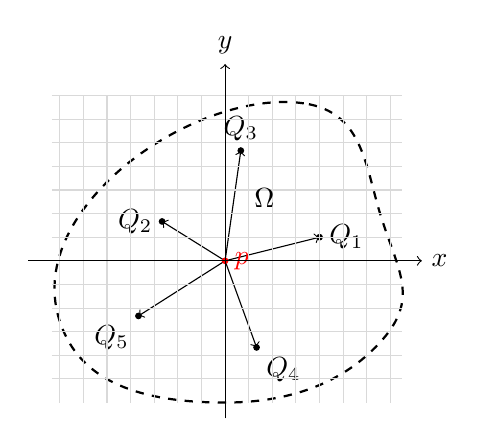
\begin{tikzpicture}
  % Define the irregular grid points
  \coordinate (p) at (0,0);
  \coordinate (Q1) at (1.2,0.3);
  \coordinate (Q2) at (-0.8,0.5);
  \coordinate (Q3) at (0.2,1.4);
  \coordinate (Q4) at (0.4,-1.1);
  \coordinate (Q5) at (-1.1,-0.7);

  % Connect central point to all other points
  \foreach \i in {1,...,5}
  \draw[->] (p) -- (Q\i);

  % Draw the points
  \filldraw[above, red] (p) circle (1pt) node[right] {$p$};
  \filldraw[black] (Q1) circle (1pt) node[right] {$Q_1$};
  \filldraw[black] (Q2) circle (1pt) node[left] {$Q_2$};
  \filldraw[black] (Q3) circle (1pt) node[above] {$Q_3$};
  \filldraw[black] (Q4) circle (1pt) node[below right] {$Q_4$};
  \filldraw[black] (Q5) circle (1pt) node[below left] {$Q_5$};

  % Draw boundary (irregular shape)
  \draw[thick, dashed] plot [smooth cycle, tension=0.8]
  coordinates {(2,0.5) (1,2) (-1.5,1) (-2,-1) (0,-1.8) (2,-1)};
  % grid inside the domain
  \draw[step=0.3cm,gray!30] (-2.2,-1.8) grid (2.25,2.1);

  % Label the domain
  \node at (0.5,0.8) {$\Omega$};

  % Add a coordinate system
  \draw[->] (-2.5,0) -- (2.5,0) node[right] {$x$};
  \draw[->] (0,-2) -- (0,2.5) node[above] {$y$};
\end{tikzpicture}


Now we want to find:
\[
  \mathcal{L}_h U_p = -\alpha_{pp} U_p + \sum_{i=1}^{s_p} \alpha_{pQ_i} U_{Q_i}
\]

Then we require:
\[
  \mathcal{L}u_p = \mathcal{L}_h u_p - \tau_p
\]

For consistency, we need:
\[
  \tau_p = \mathcal{O}(h^q) \quad \text{for some } q \geq 1
\]

\begin{align*}
  Q_i & = (x_p + \xi_i h, y_p + \eta_i h) \quad \text{where } \xi_i, \eta_i \in [-1,1] \text{ usually} \\
  p = (x_p, y_p)                                                                                       \\
\end{align*}
\emph{Taylor expansions} around \(p\):
\begin{align*}
  \mathcal{L}_h u_p & = -\alpha_{pp} u_p + \sum_{i=1}^{s_p} \alpha_{pQ_i} u(x_p + \xi_i h, y_p + \eta_i h)                                                                                                                                                            \\
                    & = -\alpha_{pp} u_p + \sum_{i=1}^{s_p} \alpha_{pQ_i} \left( u_p + \xi_i h u_x + \eta_i h u_y + \frac{h^2}{2} (\xi_i^2 u_{xx} + 2\xi_i\eta_i u_{xy} + \eta_i^2 u_{yy})\right) + \mathcal{O}(h^3)                                                  \\
                    & = \underbrace{\left(-\alpha_{pp}+ \sum \alpha_{pQ_i}\right)}_{k_p} u_p + \underbrace{\left(\sum \alpha_{pQ_i} \xi_i h \right)}_{d_p} u_x + \underbrace{\left(\sum \alpha_{pQ_i} \eta_i h \right)}_{e_p} u_y                                     \\
                    & + \underbrace{\frac{h^2}{2} \left(\sum \alpha_{pQ_i} \xi_i^2\right)}_{a_p} u_{xx} + \underbrace{h^2\left(\sum \alpha_{pQ_i} \xi_i\eta_i\right)}_{b_p} u_{xy} + \underbrace{\frac{h^2}{2} \left(\sum \alpha_{pQ_i} \eta_i^2\right)}_{c_p} u_{yy}
  + \mathcal{O}(h^3)
\end{align*}

\begin{definition}{Diagonal dominant matrix}{diagdominant}
  A matrix \(A\) is \emph{diagonally dominant} if
  \[
    |a_{ii}| \geq \sum_{j \neq i} |a_{ij}| \quad \forall i.
  \]

\end{definition}

In our case, we have:

\begin{align*}
  -\alpha_{pp} & = \sum_{i=1}^{s_p} \alpha_{pQ_i} - k_p \quad \text{is diagonally dominant if} \quad k_p >0 \\
\end{align*}

\subsubsection{Boundary conditions}

\paragraph{Dirichlet boundary conditions}
\begin{align*}
  W^\prime & = (x_p + h \xi , y_p) \\
  N^\prime & = (x_p, y_p + h \eta) \\
\end{align*}

We already know \(U_{W^\prime} = g(x_p + h \xi, y_p)\) and \(U_{N^\prime} = g(x_p, y_p + h \eta)\).

Now we solve for:
\begin{align*}
  \Delta u         & = \partial_x^2 u + \partial_y^2 u = f                                         \\
                   & U_S + U_N + U_W + U_E - 4U_p \quad \text{if } S,N,W,E \in \mathbb{G}          \\
  \partial_x^2 u_p & = -\alpha_p u_p + \alpha_{W^\prime}u_{W^\prime} + \alpha_E u_E - \tau_p^\star \\
  \partial_y^2 u_p & = -\beta_p u_p + \beta_{N^\prime}u_{N^\prime} + \beta_S u_S - \tau_N^\star
\end{align*}

where:
\begin{align*}
  \alpha_{W^\prime} & = \frac{2}{h^2}\frac{1}{\xi (\xi + 1)},   &
  \alpha_E          & = \frac{2}{h^2}\frac{1}{\xi + 1},         &
  \alpha_p          & = \frac{2}{h^2}\frac{1}{\xi}                \\
  \beta_{N^\prime}  & = \frac{2}{h^2}\frac{1}{\eta + 1},        &
  \beta_S           & = \frac{2}{h^2}\frac{1}{\eta (\eta + 1)}, &
  \beta_p           & = \frac{2}{h^2}\frac{1}{\eta}
\end{align*}

The truncation error is:
\begin{align*}
  \tau_p & = \tau_p^\star + \tau_N^\star = \frac{h}{3}\left[(1-\xi)\partial_x^3 u_p + (1-\eta)\partial_y^3 u_p\right] + \mathcal{O}(h^2)
\end{align*}

With consistency and non-negativity conditions:
\begin{align*}
  \alpha_{pQ_i} & \geq 0, \quad \alpha_{p^2} \geq 0                  \\
  \alpha_{pp}   & = \sum_{i=1}^{s_p} \alpha_{pQ_i} \tag{consistency}
\end{align*}

\paragraph{Neumann boundary conditions}
\begin{align*}
  \frac{\partial u}{\partial \vec{n}}   & = g \text{ on } \partial\Omega_N \subset \partial\Omega                                                                                                                     \\
  \vec{n}                               & = \left[n_x, n_y\right], \quad \frac{\partial u_p}{\partial \vec{n}} = n_x \frac{\partial u_p}{\partial x} + n_y \frac{\partial u_p}{\partial y} = \vec{n} \cdot \nabla u_p \\
  \frac{\partial u_p}{\partial \vec{n}} & = \frac{1}{d}\left[u_{Q^\prime} - u_p\right] + \mathcal{O}(d)                                                                                                               \\
  u_{Q^\prime}                          & = u_R + \frac{h^\prime}{h}\left(u_Q - u_R\right) + \mathcal{O}(h^2)                                                                                                         \\
  g_p                                   & = \frac{1}{d}\left(U_R + \frac{h^\prime}{h}\left(U_Q - U_R\right) - U_p\right), \quad \tau_p \approx \mathcal{O}(h)                                                         \\
  B_n U_p                               & = \frac{1}{d}\left(-U_p + (1-\frac{h^\prime}{h})U_R + \frac{h^\prime}{h}U_Q\right)                                                                                          \\
  \alpha_{pp}                           & = \frac{1}{d}, \quad \alpha_{pR} = \frac{1}{d}\left(1-\frac{h^\prime}{h}\right), \quad \alpha_{pQ} = \frac{1}{d}\frac{h^\prime}{h}                                          \\
  \alpha_{pp}                           & = \alpha_{pR} + \alpha_{pQ}                                                                                                                                                 \\
  0 \le                                 & h^\prime \le h \implies \alpha_{pR}, \alpha_{pQ} \ge 0
\end{align*}

\subsubsection{What we should know for FDM's}

In FDM with elliptic problems we should know how to (Linear equations):
\begin{itemize}
  \item Given the PDE, Domain\(\Omega\), and boundary conditions \(\partial\Omega\).
  \item Given a grid \(\mathbb{G}\).
  \item Construct the scheme \(\mathcal{L}_h U_p\).
  \item Fint the local truncation error \(\tau_p\).
  \item Error an error analysis.
  \item Implementation of the scheme.
\end{itemize}

\
\section{Forelesning 17 (Mandag 3. mars 2025) \texorpdfstring{\color{red}{Ikke møtt}}{Ikke møtt}}
\section{Forelesning 18 (Tirsdag 4. mars 2025)}
Given the (PDE) \(-u_{xx} = f\) on \(\Omega = (0,1)\) with boundary conditions \(u(0) = u(1) = 0\).
\begin{itemize}
  \item Multiply by a test function \(v\).
  \item Integrate over the domain \(\Omega\).
  \item Use partial integration to get rid of the second derivative \(u_{xx}\).
\end{itemize}
\begin{align*}
  \int_0^1 -u_{xx} v \,dx                          & = \int_0^1 f v \,dx \\
  -\int_0^1 u_x v_x \,dx + [u_x v]_0^1             & = \int_0^1 f v \,dx \\
  -\int_0^1 u_x v_x \,dx + u_x(1)v(1) - u_x(0)v(0) & = \int_0^1 f v \,dx \\
  -\int_0^1 u_x v_x \,dx                           & = \int_0^1 f v \,dx
\end{align*}

If we choose \(v\) s.t. \(v(0) = v(1) = 0\), we need to find:
\[
  \boxed{\text{find } u\in V \quad \text{s.t.} \quad \int_0^1 u_x v_x \,dx = \int_0^1 f v \,dx \forall v\in V}
\]

But how do we choose \(V\)? The integrals should exist!
\[
  f \in \mathrm{L}^2(\Omega), \quad v \in \mathrm{L}^2(\Omega), \quad u_x, v_x \in \mathrm{L}^2(\Omega)
\]

Then we can choose \(V = \mathrm{H}^1(\Omega)\), which is the Sobolev space of functions with square integrable derivatives and vanishing boundary values.

\begin{align*}
  \mathrm{H}^1_0 (\Omega) & = \{v\in \mathrm{H}^1(\Omega) \mid  v(0) = v(1) = 0\} \\
  \mathrm{H}^1(\Omega)    & = \{v \mid v, v_x \in \mathrm{L}^2(\Omega)\}
\end{align*}

\(\mathrm{H}^1(\Omega)\) and \(\mathrm{H}^1_0 (\Omega)\) are Hilbert spaces with the inner product:
\[
  \langle u, v \rangle_{\mathrm{H}^1(\Omega)} = \int_0^1 u v \,dx + \int_0^1 u_x v_x \,dx = \langle u, v \rangle_{\mathrm{L}^2(\Omega)} + \langle u_x, v_x \rangle_{\mathrm{L}^2(\Omega)}
\]
\(\mathrm{H}^1_0 (\Omega)\) is a closed subspace of \(\mathrm{H}^1(\Omega)\):
\[
  \mathrm{H}^1_0 (\Omega) \subset \mathrm{H}^1(\Omega)
\]

We also have a \emph{norm} defined by:
\[
  \norm*{v}_{\mathrm{H}^1(\Omega)}^2 = \langle v, v \rangle_{\mathrm{H}^1(\Omega)} = \norm*{v}_{\mathrm{L}^2}^2 + \norm*{v_x}_{\mathrm{L}^2}^2 = \int_0^1 v^2 \,dx + \int_0^1 v_x^2 \,dx
\]

\begin{itemize}
  \item \textbf{Semi-norm:} Since \(\abs*{v}_{\mathrm{H}^1}^2 = \norm*{v_x }_{\mathrm{L}^2}^2\) can be zero, it is called a semi-norm.
  \item If \(v\in \mathrm{H}^1(\Omega)\), then \(v\) is \textbf{continuous}.
\end{itemize}

\subsection{Abstract Formulation}
\[
  \boxed{\text{Find }u\in V\text{ s.t. }a(u,v) = F(v)\text{ for all }v\in V}
\]
where \(\symbf{v}\) is the test function and \(\symbf{u}\) is the trial function (solution).

Let \(V = \mathrm{H}^1_0 (\Omega)\) and \(\Omega = (0,1)\).
\[
  a(u,v) = \langle u_x, v_x \rangle_{\mathrm{L}^2} = \int_0^1 u_x v_x \,dx
\]
\[
  F(v) = \langle f, v \rangle_{\mathrm{L}^2} = \int_0^1 f v \,dx
\]
\begin{theorem}{Lax-Milgram}{laxmilgram}
  Let \(V\) be a \emph{Hilbert space} with inner product \(\inner{\cdot, \cdot}\) and norm \(\norm*{\cdot}_V\). Let \(a: V\times V\to \R\) be a bilinear form and \(F: V\to \R\) be a linear functional. If:
  \begin{itemize}
    \item \(a(u,v)\) is continuous and bilinear in \(u\) and \(v\):
          \[
            |a(u,v)| \leq C_a \norm*{u}_V\norm*{v}_V
          \]
    \item \(a(u,u)\) is coercive in \(u\):
          \[
            a(u,u) \geq C_c\norm*{u}_V^2
          \]
    \item \(F(v)\) is continuous or linear in \(v\):
          \[
            |F(v)| \leq C_F\norm*{v}_V
          \]
  \end{itemize}
  Where \(C_a, C_c, C_F > 0\).

  \medskip

  Then there exists a unique solution \(u\in V\) to the problem:
  \[
    a(u,v) = F(v), v\in V
  \]
  and the solution satisfies:
  \[
    C_c^{-1}C_a^{-1}C_F^2
  \]
\end{theorem}

\section{Forelesning 21 (Mandag 11. mars 2025)}

\subsection{Finite Element Method (FEM)}

\begin{itemize}
  \item Find $u\in V$ s.t. \(a(u,v) = F(v)\) for all \(v\in V\).
  \item Find $u\in V_h$ s.t. \(a(u_h,v) = F(v)\) for all \(v\in V_h\), when \(V_h\in\spann\{\phi_1,\phi_2,\dots,\phi_n\}\).
  \item Solve \(A\vec{u} = \vec{f}\) for \(\vec{u}\), where
        \[
          A_{ij} = a(\phi_i,\phi_j), \quad \vec{f}_i = F(\phi_i)
        \]
\end{itemize}

\subsection{Finite Element Space}
Let's construct a finite element space on a one-dimensional domain:

\begin{itemize}
  \item First, we partition the domain $\Omega = [0,1]$ into $M$ subintervals:
        \[
          0 = x_0 < x_1 < \dots < x_{M-1} < x_M = 1
        \]
  \item Each subinterval $K_j = [x_j, x_{j+1}]$ for $j = 0,1,\dots,M-1$ forms an element.
  \item The length of each element is $h_j = x_{j+1} - x_j$. For uniform meshes, $h_j = h = \frac{1}{M}$.
  \item We define the finite element space $V_h^r$ as:
        \[
          V_h^r = \{v \in C^0([0,1]) : v|_{K_j} \in \mathbb{P}_r \text{ for all } j,\, v(0) = v(1) = 0\}
        \]
        where $\mathbb{P}_r$ is the space of polynomials of degree $\leq r$.
  \item This space $V_h^r \subset H^1_0(\Omega)$ consists of continuous, piecewise polynomial functions that vanish at the boundary.
\end{itemize}

\begin{figure}[H]
  \centering
  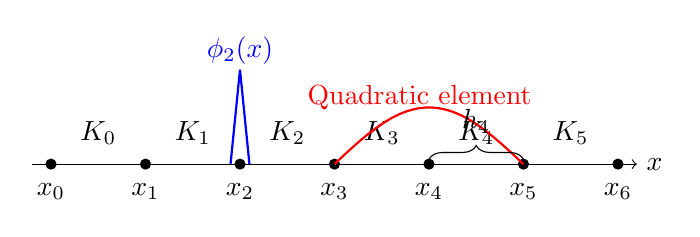
\begin{tikzpicture}[scale=1.2]
    % Draw x-axis with nodes
    \draw[->] (-0.2,0) -- (6.2,0) node[right] {$x$};

    % Draw nodes/grid points
    \foreach \x/\i in {0/0, 1/1, 2/2, 3/3, 4/4, 5/5, 6/6} {
        \filldraw[black] (\x,0) circle (1.5pt);
        \node[below] at (\x,-0.1) {$x_{\i}$};
      }

    % Label elements
    \foreach \x/\i in {0.5/0, 1.5/1, 2.5/2, 3.5/3, 4.5/4, 5.5/5} {
        \node[above] at (\x, 0.1) {$K_{\i}$};
      }

    % Example of linear basis function
    \draw[thick, blue] (1.9,0) -- (2,1) -- (2.1,0);
    \node[blue] at (2,1.2) {$\phi_2(x)$};

    % Another example for higher-order basis
    \draw[thick, red, domain=3:5, samples=30] plot (\x, {0.6*sin((\x-3)*180/2)});
    \node[red] at (3.9,0.7) {Quadratic element};

    % Draw a brace for h_j
    \draw[decorate, decoration={brace, amplitude=5pt}] (4,0.05) -- (5,0.05) node[midway, above=6pt] {$h_4$};
  \end{tikzpicture}
  \caption{Partition of domain into finite elements with examples of basis functions}
\end{figure}

\subsection{Basis Functions}
For $r=1$ (linear elements), we can construct a basis explicitly:

\begin{itemize}
  \item Define "hat functions" $\phi_j(x)$ for $j = 1,2,\dots,M-1$:
        \[
          \phi_j(x) =
          \begin{cases}
            \frac{x - x_{j-1}}{h_{j-1}} & \text{if } x \in [x_{j-1}, x_j] \\
            \frac{x_{j+1} - x}{h_j}     & \text{if } x \in [x_j, x_{j+1}] \\
            0                           & \text{otherwise}
          \end{cases}
        \]
  \item These functions satisfy: $\phi_j(x_i) = \delta_{ij}$ (equals 1 at node $j$ and 0 at all other nodes).
  \item The space $V_h^1 = \text{span}\{\phi_1, \phi_2, \ldots, \phi_{M-1}\}$.
  \item For a function $u_h \in V_h^1$, we can write:
        \[
          u_h(x) = \sum_{j=1}^{M-1} u_j \phi_j(x)
        \]
        where $u_j = u_h(x_j)$ are the nodal values (degrees of freedom).
\end{itemize}

\begin{figure}[H]
  \centering
  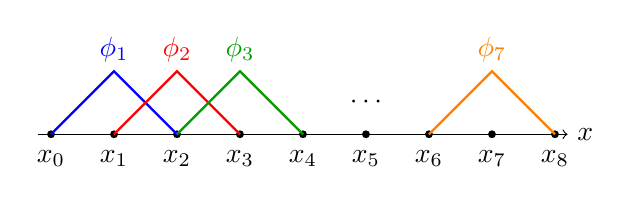
\begin{tikzpicture}[scale=0.8]
    % Draw x-axis
    \draw[->] (-0.2,0) -- (8.2,0) node[right] {$x$};

    % Draw nodes
    \foreach \x/\i in {0/0, 1/1, 2/2, 3/3, 4/4, 5/5, 6/6, 7/7, 8/8} {
        \filldraw[black] (\x,0) circle (1.5pt);
        \node[below] at (\x,-0.1) {$x_{\i}$};
      }

    % Draw hat functions
    \draw[thick, blue] (0,0) -- (1,1) -- (2,0);
    \node[blue, above] at (1,1) {$\phi_1$};

    \draw[thick, red] (1,0) -- (2,1) -- (3,0);
    \node[red, above] at (2,1) {$\phi_2$};

    \draw[thick, green!60!black] (2,0) -- (3,1) -- (4,0);
    \node[green!60!black, above] at (3,1) {$\phi_3$};

    \draw[thick, orange] (6,0) -- (7,1) -- (8,0);
    \node[orange, above] at (7,1) {$\phi_7$};

    % Draw dots to indicate more basis functions
    \node at (5,0.5) {$\cdots$};
  \end{tikzpicture}
  \caption{Linear basis functions (hat functions) for the finite element space $V_h^1$}
\end{figure}

\subsection{Higher Order Elements}
For $r > 1$, we need additional basis functions:

\begin{itemize}
  \item For quadratic elements ($r=2$), we introduce additional nodes at the midpoints $x_{j+1/2} = \frac{x_j + x_{j+1}}{2}$.
  \item Each element then has 3 nodes: two endpoints and one midpoint.
  \item The basis consists of quadratic functions, allowing for more accurate approximations.
  \item The dimension of $V_h^2$ is $2M-1$ (with $M-1$ vertex nodes and $M$ midpoint nodes).
\end{itemize}

\begin{figure}[H]
  \centering
  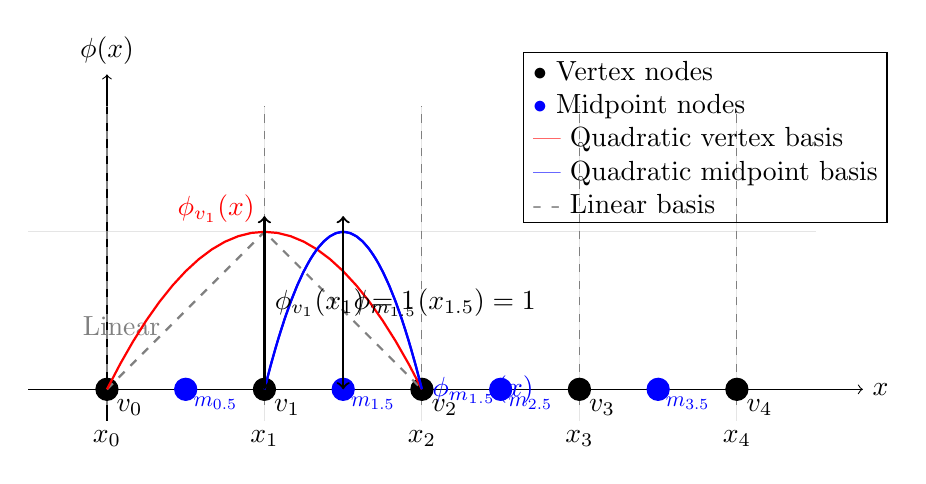
\begin{tikzpicture}[scale=2.0]
    % Grid and axes
    \draw[step=1cm,gray!20] (-0.5,-0.2) grid (4.5,1.8);
    \draw[->] (-0.5,0) -- (4.8,0) node[right] {$x$};
    \draw[->] (0,-0.2) -- (0,2) node[above] {$\phi(x)$};

    % Element boundaries
    \foreach \x in {0,1,2,3,4} {
        \draw[dashed, gray] (\x,-0.1) -- (\x,1.8);
        \node[below] at (\x,-0.2) {$x_{\x}$};
      }

    % Nodes with different styles
    \foreach \x in {0,1,2,3,4} {
        \filldraw[black] (\x,0) circle (2pt) node[below right] {$v_{\x}$};
      }

    % Midpoint nodes
    \foreach \x/\i in {0.5/0.5, 1.5/1.5, 2.5/2.5, 3.5/3.5} {
        \filldraw[blue] (\x,0) circle (2pt) node[below right, scale=0.8] {$m_{\i}$};
      }

    % Linear basis function (for comparison)
    \draw[thick, gray, dashed, domain=0:2] plot (\x, {max(0,1-abs(\x-1))});
    \node[gray, left] at (0.4,0.4) {Linear};

    % Quadratic basis function at vertex x_1
    \draw[thick, red, domain=0:2] plot (\x, {\x*(2-\x)});
    \node[red, above left] at (1,1) {$\phi_{v_1}(x)$};

    % Quadratic basis function at midpoint x_1.5
    \draw[thick, blue, domain=1:2] plot (\x, {4*(\x-1)*(2-\x)});
    \draw[thick, blue, domain=1:2, samples=30] plot (\x, {4*(\x-1)*(2-\x)}) node[right, blue] at (2,0) {$\phi_{m_{1.5}}(x)$};

    % Annotations
    \draw[<->, thick] (1,1.1) -- (1,0) node[midway, right] {$\phi_{v_1}(x_1)=1$};
    \draw[<->, thick] (1.5,1.1) -- (1.5,0) node[midway, right] {$\phi_{m_{1.5}}(x_{1.5})=1$};

    % Legend
    \node at (3.8,1.6) [draw, align=left] {
      \textcolor{black}{$\bullet$} Vertex nodes\\
      \textcolor{blue}{$\bullet$} Midpoint nodes\\
      \textcolor{red}{—} Quadratic vertex basis\\
      \textcolor{blue}{—} Quadratic midpoint basis\\
      \textcolor{gray}{- -} Linear basis
    };
  \end{tikzpicture}
  \caption{Comparison of linear and quadratic basis functions. The quadratic elements use additional midpoint nodes, allowing for curved functions that provide higher accuracy. Each basis function equals 1 at its corresponding node and 0 at all other nodes.}
\end{figure}

\subsection{Assembly of the Linear System}
To compute the solution $u_h \in V_h^r$, we need to:

\begin{itemize}
  \item Express $u_h = \sum_{j=1}^N U_j \phi_j(x)$, where $N$ is the dimension of $V_h^r$.
  \item For linear elements on a uniform mesh, $N = M-1$.
  \item Insert this into the variational form: Find $u_h \in V_h^r$ such that
        \[
          a(u_h, v_h) = F(v_h) \quad \forall v_h \in V_h^r
        \]
  \item Testing with each basis function $\phi_i$ leads to a linear system:
        \[
          \sum_{j=1}^N a(\phi_j, \phi_i) U_j = F(\phi_i), \quad i = 1,2,\ldots,N
        \]
  \item The resulting system matrix $A_{ij} = a(\phi_j, \phi_i)$ is sparse, as basis functions with non-overlapping support lead to zero entries.
\end{itemize}

For our model problem with $a(u,v) = \int_0^1 u_x v_x \, dx$, we compute:

\[
  A_{ij} = a(\phi_j, \phi_i) = \int_0^1 \phi_j'(x) \phi_i'(x) \, dx
\]

For linear elements, this can be computed explicitly, yielding a tridiagonal matrix.

\subsection{Reference Element \texorpdfstring{$\hat{K}$}{K}}

In the finite element method, a powerful technique is to define shape functions and perform calculations on a standard "reference element" $\hat{K}$ rather than on each physical element. This simplifies implementation and numerical integration.

\subsubsection{Reference Element in 1D}
For one-dimensional problems, we typically choose the reference element as:
\[
  \hat{K} = [0,1]
\]

\paragraph{Affine Mapping}
Each physical element $K_j = [x_j, x_{j+1}]$ can be mapped to the reference element $\hat{K}$ through an affine transformation:
\[
  F_j(\hat{x}) = x_j + h_j\hat{x}
\]
where $\hat{x} \in [0,1]$ is the coordinate in the reference element, and $h_j = x_{j+1} - x_j$ is the length of the physical element.

The inverse mapping is:
\[
  F_j^{-1}(x) = \frac{x - x_j}{h_j}
\]

\paragraph{Shape Functions on the Reference Element}
Instead of defining shape functions directly on each element, we define them once on the reference element:

\begin{itemize}
  \item Linear shape functions on $\hat{K}$:
        \[
          \hat{\phi}_0(\hat{x}) = 1-\hat{x}, \quad \hat{\phi}_1(\hat{x}) = \hat{x}
        \]

  \item Quadratic shape functions on $\hat{K}$:
        \[
          \hat{\phi}_1(\hat{x}) = -4\hat{x}^2 + 4\hat{x}, \quad
          \hat{\phi}_2(\hat{x}) = 2\hat{x}^2 - \hat{x}
        \]
\end{itemize}

\paragraph{Mapping Shape Functions}
The shape functions on a physical element are defined via the reference element as:
\[
  \phi_j(x) = \hat{\phi}_j(F_j^{-1}(x)) \quad \text{for } x \in K_j
\]
where $j$ indicates the element number. The shape functions $\phi_j(x)$ are piecewise linear or quadratic functions that are non-zero only on the element $K_j$.
\begin{align*}
  \phi_j(x)     & = \hat{\phi}_j(F_j^{-1}(x))     \\
  \phi_{j+1}(x) & = \hat{\phi}_{j+1}(F_j^{-1}(x))
\end{align*}

\begin{figure}[H]
  \centering
  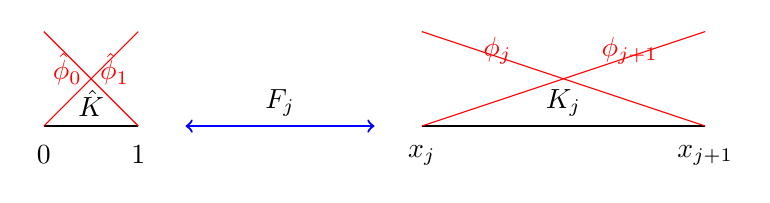
\begin{tikzpicture}[scale=1.2]
    % Reference element
    \draw[thick] (0,0) -- (1,0);
    \node[below] at (0,-0.1) {$0$};
    \node[below] at (1,-0.1) {$1$};
    \node[above] at (0.5,0) {$\hat{K}$};

    % Physical element
    \draw[thick] (4,0) -- (7,0);
    \node[below] at (4,-0.1) {$x_j$};
    \node[below] at (7,-0.1) {$x_{j+1}$};
    \node[above] at (5.5,0) {$K_j$};

    % Mapping arrow
    \draw[<->, thick, blue] (1.5,0) -- (3.5,0);
    \node[above] at (2.5,0) {$F_j$};

    % Linear shape functions on reference
    \draw[red, domain=0:1, samples=20] plot (\x, {1-\x});
    \draw[red, domain=0:1, samples=20] plot (\x, {\x});

    % Corresponding shape functions on physical element
    \draw[red, domain=4:7, samples=20] plot (\x, {(7-\x)/3});
    \draw[red, domain=4:7, samples=20] plot (\x, {(\x-4)/3});

    % Labels
    \node[red] at (0.25,0.6) {$\hat{\phi}_0$};
    \node[red] at (0.75,0.6) {$\hat{\phi}_1$};
    \node[red] at (4.8,0.8) {$\phi_j$};
    \node[red] at (6.2,0.8) {$\phi_{j+1}$};
  \end{tikzpicture}
  \caption{Mapping between reference element $\hat{K}$ and physical element $K_j$}
\end{figure}

\paragraph{Integration Using Reference Element}
When computing element matrices and vectors, we transform integrals over physical elements to integrals over the reference element:
\[
  \int_{K_j} f(x)\,dx = \int_{\hat{K}} f(F_j(\hat{x}))|J_j|\,d\hat{x}
\]
where $|J_j| = h_j$ is the determinant of the Jacobian of the mapping.

For our model problem, the element stiffness matrix entries become:
\[
  A_{ij}^K = \int_{K} \phi_i'(x)\phi_j'(x)\,dx = \int_{\hat{K}} \hat{\phi}_i'(\hat{x})\hat{\phi}_j'(\hat{x})\frac{1}{h_K}\,d\hat{x}
\]


\paragraph{Advantages}
\begin{itemize}
  \item Quadrature rules need to be defined only once on the reference element
  \item Shape functions and their derivatives are pre-computed on $\hat{K}$
  \item Code structure becomes simpler and more modular
  \item Easily extends to higher dimensions and higher-order elements
\end{itemize}

\begin{example}{Linear Element Computation}{}
  For linear elements with $\hat{\phi}_0(\hat{x}) = 1-\hat{x}$ and $\hat{\phi}_1(\hat{x}) = \hat{x}$:

  \begin{align*}
    \hat{\phi}_0'(\hat{x}) & = -1 \\
    \hat{\phi}_1'(\hat{x}) & = 1
  \end{align*}

  The element stiffness matrix on the reference element is:
  \[
    \hat{A} = \int_0^1
    \begin{bmatrix}
      (-1)(-1) & (-1)(1) \\
      (1)(-1)  & (1)(1)
    \end{bmatrix}
    \, d\hat{x} =
    \begin{bmatrix}
      1  & -1 \\
      -1 & 1
    \end{bmatrix}
  \]

  For a physical element $K_j$ of length $h_j$, the element stiffness matrix is:
  \[
    A^{K_j} = \frac{1}{h_j}\hat{A} = \frac{1}{h_j}
    \begin{bmatrix}
      1  & -1 \\
      -1 & 1
    \end{bmatrix}
  \]

  This approach forms the foundation for efficient implementation of finite element methods across different element types and problem dimensions.
  
  \begin{align*}
    \phi_j^K(x)           & = \hat{\phi}_j(F_K^{-1}(x)) \\
    \hat{\phi}_0(\hat{x}) & = 2\hat{x}^2 - 3\hat{x} + 1
  \end{align*}
\end{example}
